% Journal of Aircraft review-format draft. Not yet submission-ready.
% AIAA minimum: US letter, 10-point, single column, double-spaced.
\documentclass[10pt,letterpaper]{article}
\usepackage[T1]{fontenc}
\usepackage{mathptmx}
\usepackage[margin=1in]{geometry}
\usepackage{amsmath,amssymb,graphicx,booktabs,tabularx,array,float,pdflscape}
\usepackage{microtype}
\usepackage[hidelinks]{hyperref}
\usepackage{xurl}
\usepackage[font=small,labelfont=bf]{caption}
\linespread{1.667}\selectfont
\setlength{\emergencystretch}{5em}
\setlength{\tabcolsep}{4pt}
\renewcommand{\arraystretch}{1.16}
\newcommand{\figdir}{figures}
\title{Auditing Historically Constrained Language-Model Aircraft Against the Wright Flyer}
\author{Ehsan Roohi\\
\small Department of Mechanical and Industrial Engineering\\
\small University of Massachusetts Amherst, Amherst, MA 01003, USA\\
\small Corresponding author: \texttt{roohie@umass.edu}}
\date{}
\begin{document}
\maketitle

\begin{abstract}
Three language models were asked to design piloted, powered aircraft using a shared packet of aviation sources dated no later than 1898. Their proposals and subsequent revisions were independently audited for geometry, mass, force and moment balance, propulsion assumptions, and local stability. Initial concepts exposed destabilizing pitch response, interfering controls, or insufficiently supported power targets. Later feedback and corrected evaluator geometry produced a Fable candidate with positive conditional longitudinal margins of 3.98--10.12\% across eight loading states at 13 m/s. These results describe rigid lifting surfaces, not installed-aircraft trim. Replacing the response's induced-drag estimate with the corresponding surface calculation reduces the heavy-case power reserve at 13 m/s to 11.0\%, below the exploratory 15\% target. At 12 m/s the conditional reserve increases to 22.5\%, but stall margin is unknown; at 16 m/s the assumed power deficit is 5.99 kW. Propeller refinement and engine-assumption checks similarly qualify the other two proposals. No design has demonstrated whole-aircraft balance, validated dynamic modes, or structural adequacy. Comparison with successive Wright aircraft distinguishes observed pilot-controlled flight from passive restoring tendencies and emphasizes evidence-producing iteration rather than plausible geometry.
\end{abstract}

\section*{Nomenclature}
\noindent\begin{tabular}{@{}ll@{}}
$C_{m_\alpha}$ & fixed-control pitching-moment slope, rad$^{-1}$\\
$C_{m_q}$ & pitch-rate pitching-moment derivative, nondimensional\\
$C_Y,C_l,C_n$ & side-force, rolling-moment and yawing-moment coefficients\\
$\beta$ & sideslip angle, rad unless otherwise stated\\
$\delta_{\rm tip},\delta_r$ & commanded tip-panel and rudder rotations\\
$D$ & installed aircraft drag, N\\
$L$ & lift, N\\
$P_e$ & engine-side output power, W\\
$P_{\mathrm{shaft}}$ & power at propeller shafts, W\\
$V$ & flight speed, m/s (not a design-version label)\\
$\eta_g$ & engine-to-propeller drive efficiency\\
$\eta_p$ & useful-to-propeller-shaft efficiency\\
\end{tabular}

\section{Introduction}
An aircraft proposal is not a flight demonstration. A configuration can look plausible, produce sufficient nominal lift, and still fail because its pitching moments cannot be balanced, its controls cannot move through the required travel, or its installed propulsion cannot overcome total drag. This distinction becomes especially important when a language model generates a technically fluent account alongside an attractive drawing. The question examined here is not whether models can name aircraft components, but whether the components they specify form an evaluable, coupled engineering system.

The Wright Flyer offers a demanding historical comparison, provided the comparison is not reduced to a contest between silhouettes. Chanute's account of nineteenth-century experiments already treated equilibrium, propulsion, materials, and practical operation as interconnected problems \cite{ref1}. Wilbur Wright's 1901 lecture describes disappointing lift predictions, experiments with the center of pressure, and changes to the apparatus \cite{ref2}. The surviving first-flight photograph documents an operating machine and pilot rather than a proposed configuration \cite{ref4}. Culick's engineering history places the Wrights' accomplishment in their combined work as designers and test pilots \cite{ref5}. The relevant comparison is therefore between evidence-producing design processes, not between the eloquence of their explanations.

The brothers' route to the powered Flyer was a sequence of tests and revisions, not a single inspired drawing. They explored wing deformation for roll control, flew successive gliders, found that inherited lift predictions were unreliable, measured wing models in their own wind tunnel, and used the results in the 1902 glider before integrating a light engine and two propellers in 1903 \cite{ref2,ref35}. The prone pilot reduced frontal resistance; the forward horizontal surface controlled pitch as the aerodynamic load moved; wing warping and a linked vertical rudder addressed roll and yaw together. The rear propellers, chain transmission, engine, structure and launch apparatus then had to work as one system. None of these features alone guaranteed safe flight. Their relevance here is methodological: each proposed arrangement must be exposed to mass, lift, moment, power, control and structural checks, followed by a recorded change when a check fails. The models were not given knowledge of the later Wright experiments as design input; this comparison was performed afterwards.

Studies of historical aircraft show what is needed to move beyond a plausible reconstruction. Full-scale tests of the 1901 glider examined cloth treatment and ground-effect conditions \cite{ref8}. Analyses of the 1902 glider connected aerodynamic information with flight-control development and handling qualities \cite{ref7,ref9}. Deters, Broughton, and Selig developed distinct simulation representations for the 1903 and 1905 Flyers rather than treating all Wright configurations as interchangeable \cite{ref11}. The Ames replica project and its full-scale tests provide further evidence, but that replica and its test configuration must be distinguished from the 1903 aircraft \cite{ref12,ref13}.

Recent \emph{Journal of Aircraft} studies of Lilienthal's machines follow a similarly explicit chain from historical interpretation through reconstruction and measurement to constrained flight evidence. Raffel and colleagues investigated stability and controllability of the 1893 monoplane \cite{ref16}, the flying qualities of the large biplane \cite{ref17}, and individual control mechanisms of the 1895 experimental monoplane \cite{ref18}. Their results concern specified configurations and tested functions. They do not convert an untested device into a validated one merely because it is shown in a drawing. Separate wind-tunnel work also identifies fabric properties as an aerodynamic variable \cite{ref19}. These studies motivate the present separation of geometric definition, numerical prediction, and physical evidence.

Language-model-assisted aircraft design is already an active research topic. Tong et al. compare prompting approaches and generated aircraft concepts with engineering designs \cite{ref25}; their publisher abstract establishes a direct conceptual-design precedent, but does not by itself support conclusions about every validation step in that study. Krus examines aircraft-system design and simulation-code assistance, including corrective interaction \cite{ref26}. The iDesignGPT study evaluates an agentic conceptual-design workflow, including an aircraft challenge \cite{ref27}. AGENT explores structured aerial-vehicle generation \cite{ref28}, while AircraftVerse links design descriptions, geometry, and simulation-related artifacts \cite{ref29}. These different representations and evaluation endpoints should not be collapsed into a single measure of ``AI aircraft design.''

This study contributes an artifact-level engineering assessment of three historically prompted concepts. It asks: (1) what was actually specified, (2) which conditional force and moment balances can be supported, (3) what the available evidence says about stability and mechanical feasibility, and (4) which deficiencies must be addressed by a recorded feedback cycle. It does not claim the first use of language models in aircraft design, historically independent invention, or a controlled ranking of model capabilities. The three cases lack matched repeated trials and received unequal clarification budgets.

% Source-audited historical subsection for a future JoA manuscript revision.
% Keep it distinct from the V0--V2 evaluator results and the later V15 screens.
\subsection{The Wright aircraft as an evolving aerodynamic and control system}
\label{sec:wright-history-dynamics}

The 1903 Flyer is an observed flight baseline, not a certificate of passive
stability or a fixed template for the three model-generated concepts. The
Wrights' route began with kites and successive piloted gliders; shortfalls in
the 1901 lift predictions led them to measure wing shapes in their own wind
tunnel, revise the lifting surfaces, and refine three-axis control in the 1902
glider. The powered Flyer retained two fabric-covered, braced wing decks,
wing-warp roll control, a forward pitch-control surface, and a linked aft
vertical rudder. A prone pilot lay beside the engine on the lower deck, while
chains drove two counter-rotating pusher propellers. Thus a propeller or
center-of-gravity change altered an integrated aircraft rather than an
isolated subsystem \cite{ref2,ref35,ref6}.

The original structure matters aerodynamically. Wood spars, ribs, fabric,
struts, and tensioned wires supplied the load path while permitting the
intended wing warp. In a later full-scale replica test, fabric billowing
increased effective camber and changed the lift curve, and the flexible
canard showed substantially different effectiveness from smaller rigid
models. That replica was locally reinforced to accept a tunnel sting, so its
measurements are valuable but are not proof of the exact 1903 airframe's
strength or an as-flown dynamic derivative database \cite{ref13}. A proposed
historical-style aircraft must therefore report member and joint stiffness,
control-surface travel under load, and fabric/shape uncertainty, not just a
three-view outline.

Propulsion was likewise part of the balance problem. The 1903 machine used a
roughly 12-hp engine, two pusher propellers and a chain transmission; the
propellers were treated as rotating lifting surfaces, not simple flat
blades \cite{ref35,ref43}. In the 1999 full-scale replica tunnel program,
the reproduced propellers at the test stand's permitted maximum of 340 rpm
did not produce thrust equal to drag at the selected 25-knot condition.
That limitation of a particular powered replica test does not overturn the
recorded 1903 flights. It demonstrates why engine rpm, delivered shaft power,
propeller advance ratio, transmission losses and installed drag must be
matched before declaring any of the present concepts capable of level
powered flight \cite{ref13}. Historical notebook static-thrust values and
modern replica thrust measurements also refer to different apparatus and
conditions; they cannot be transplanted to a model-designed propeller
\cite{ref43}.

The subsequent Wright machines were revisions, not repetitions of Flyer I.
The 1904 Flyer II kept the broad canard-biplane arrangement but changed
camber, structure and power plant. Moving mass aft initially aggravated
pitch handling; forward ballast and later control-arm changes followed.
The 1905 Flyer III then underwent several changes in one season, including
removal of forward vertical ``blinkers,'' an enlarged canard, enlarged and
more distant aft vertical surfaces, and a transition toward more independent
rudder operation. Its longer control moment arms increased authority and
pitch damping even though the canard configuration did not become passively
stable in pitch. Treating an early 1905 short-nose configuration and the
autumn final machine as the same aircraft would erase the causal design
cycle \cite{ref41,ref42,ref10}.

In the 1905 study, the engine carried over from 1904 is reported at roughly
21 hp by that stage, driving two counter-rotating propellers; the source
does not provide an installed performance map for every 1905 revision
\cite{ref10}. A change in power or propeller design must therefore be
evaluated alongside altered wing loading, drag, center of gravity and
control moments, rather than treated as an independent ``more power'' fix.

Later canard Wright machines also cannot
be assigned the 1903 coefficients: the 1909 configuration is reported as
more pitch-unstable than 1903 in a modern reconstruction, and the move to
an aft horizontal tail around 1910 finally changed the passive-stability
architecture \cite{ref41}. No common, source-verified derivative table for
every intervening variant is claimed here.

The later production path illustrates why a recognizable Wright silhouette
is not a sufficient comparator. The 1909 Military Flyer still used a front
elevator, wing warping, an aft rudder, and two chain-driven pusher
propellers, but carried two people and had a smaller wing area and higher
speed than earlier machines \cite{ref44}. The 1910 Model B moved pitch
control to an aft elevator and dispensed with the front canard
\cite{ref41} (The Franklin Institute, ``Exploring an Original 1911 Wright Model B Airplane,'' 2022, \url{https://fi.edu/en/blog/exploring-original-1911-wright-model-b-airplane}, accessed 30 September 2026). Thus a ``Wright-like'' claim must identify the year,
loading, geometry, control linkage, and powertrain; the 1903 and 1910
aircraft do not even share the same longitudinal-control topology.

The cited studies answer different questions and should not be merged into
one purported ``Wright dataset.'' Culick and Jex analyzed the 1903
aircraft's aerodynamics, instability and pilot-in-the-loop control; their
work is a flight-mechanics reconstruction, not a direct flight-test record
of every derivative \cite{ref6}. Jex and colleagues obtained full-scale,
six-component wind-tunnel evidence from a carefully constructed but
reinforced 1903 replica, revealing fabric and canard-flexibility effects
and an unfavorable propulsion result at the tested rpm \cite{ref13}.
Padfield and Lawrence reconstructed the 1904--1905 modification cycle and
pilot handling, while Lawrence and Padfield combined 1905 tunnel data,
computed rate derivatives and piloted simulation to compare 1903 and final
1905 modes \cite{ref42,ref10}. Papachristodoulou and Culick extended the
configuration-level flight-mechanics comparison into the later canard and
aft-tail years \cite{ref41}. Ash and colleagues independently examined
historical propeller shapes and static-thrust tests; static thrust is not
an installed thrust--power--speed map \cite{ref43}. These papers justify
the kinds of evidence sought here, but none supplies the absent engine,
structure or unsteady-flow data for Astra, Fable or Opus.

\subsection{Measured derivatives, reconstructed modes, and pilot action}
\label{sec:wright-mode-baseline}

To compare signs without conflating conventions, define the conventional
fixed-control static margin as
$SM=-C_{m_\alpha}/C_{L_\alpha}$, with the derivatives evaluated at a stated
trim point and with the same reference chord. The 1905 study instead reports
$H_n=\partial C_M/\partial C_L$ as a positive \emph{magnitude of
instability}; its $H_n$ must not be read as a positive restoring margin.
Define the nondimensional pitch-rate derivative by
$C_{m_q}=\partial C_m/\partial(q\bar c/2V)$ and the corresponding
unsteady incidence-rate derivative by
$C_{m_{\dot\alpha}}=\partial C_m/\partial(\dot\alpha\bar c/2V)$.
The historical sources inspected here support selected measured slopes and
modelled rate terms, but do not provide a verified common
$C_{m_{\dot\alpha}}$ for all Wright configurations \cite{ref13,ref10,ref42}.

\begin{table}[p]
\centering\small
\caption{Selected published Wright stability quantities. Values belong to the stated replica or simulation and must not be substituted into a V15 design.}
\label{tab:wright-derivative-baseline}
\begin{tabularx}{\linewidth}{@{}p{.19\linewidth}p{.21\linewidth}p{.22\linewidth}X@{}}
\toprule
Configuration & Quantity & Reported value & Evidence and qualification\\
\midrule
1903 Flyer replica & Conventional $SM$ & about $-0.25$ ($-25\%$ MAC) & Full-scale Ames tunnel interpretation; reference CG near $0.30\bar c$, neutral point near $0.05\bar c$; approximately 25 kt \cite{ref13}.\\
1903 Flyer model & $C_{m_q}$ & about $-1.53$ & Estimated pitch damping in the Lawrence--Padfield model, not a direct 1903 in-flight measurement \cite{ref10}.\\
1903 Flyer model & unstable pitch pole; doubling time & $+1.6861\ \mathrm{s}^{-1}$; $0.41$ s & Linearized reconstruction; varies with mass and flight condition \cite{ref10}.\\
1905 final Flyer III & $C_{n_\beta}$ & $+0.0403\ \mathrm{rad}^{-1}$ & Reported final-configuration directional slope over $-16^\circ<\beta<16^\circ$ in the model/tunnel study \cite{ref10}.\\
1905 final Flyer III & $C_{m_q}$ & about $-2.62$; alternative $-4.67$ & Two published computational estimates; disagreement is retained, not averaged \cite{ref10,ref41}.\\
1905 final Flyer III & unstable pitch pole; doubling time & $+0.3162\ \mathrm{s}^{-1}$; $2.192$ s & Linearized reconstruction with slower divergence than the 1903 model despite greater static instability \cite{ref10}.\\
1905 final Flyer III & roll; Dutch roll; spiral poles & $-3.8984$; $-0.4944\pm1.2038i$; $+0.2499\ \mathrm{s}^{-1}$ & Linearized 26-kt model; the positive spiral pole remains divergent \cite{ref10}.\\
\bottomrule
\end{tabularx}
\end{table}

The 1905 analysis also gives a reported 1903 directional slope
$C_{n_\beta}\simeq+0.0368\ \mathrm{rad}^{-1}$ from the earlier Ames work;
this is a secondary transcription, not a value independently re-extracted
from the original tunnel plots \cite{ref10,ref13}. An earlier 2005 account
prints $+0.00403\ \mathrm{rad}^{-1}$ for the final 1905
$C_{n_\beta}$, whereas the later detailed study prints
$+0.0403\ \mathrm{rad}^{-1}$. Until the original figure's slope and
normalization are reconciled, numerical cross-paper comparison must flag
this factor-of-ten discrepancy rather than silently choose a value
\cite{ref42,ref10}. The intermediate 1905 directional derivatives plotted
for blinkers, canard and vertical-tail revisions are authors' estimates;
only the specified final test configuration should be called directly
measured \cite{ref10}.

These results explain how the Wrights could fly without modern eigenvalue
analysis. A positive open-loop pitch pole means a small disturbance grows
unless an external action intervenes; it does not mean that no controllable
trajectory exists. The pilot observed pitch attitude and moved the canard
continuously. In the reconstructed pilot--aircraft model, increasing
feedback could suppress the nonoscillatory pitch divergence but could also
reduce damping of another oscillatory mode, especially when perception and
muscle delay were represented. The same pitch-attitude feedback that was
tolerable in the more damped 1905 model destabilized an oscillatory mode of
the 1903 model; this is a model-based explanation of high workload, not a
reconstructed command history of a particular historical pilot
\cite{ref6,ref10,ref42}. For lateral control, wing warp produced adverse
yaw; the linked rudder helped initial correction, but tight low-speed turns
could combine sideslip, inboard-wing high incidence and a rapidly growing
spiral. The 1905 analysis attributes improved recovery to changed
rudder authority/linkage and greater control of speed during turns
\cite{ref10,ref42}. These observations are historical analysis, not
instructions to operate an untested replica.

The implication for the present experiment is methodological. For Fable V15,
the independent, power-off wing--tail AVL sweep yields a local balance at
$V=13$ m/s under assumed mass and section data and a window-sensitive
\emph{apparent} margin near $0.53$--$1.23\%$ of the reference chord.
This is not comparable in fidelity to a six-component, propeller-on Ames
replica test, and it does not supply $C_{m_{\dot\alpha}}$, validated
installed $C_{m_q}$, lateral--directional derivatives or modal roots.
Astra and Opus V15 retain independent propulsion or installation holds;
none of the three designs currently has a verified whole-aircraft trim or
accepted dynamic mode set. Our target is therefore first a physically
specified and independently checked airframe/propulsion model, next a
six-force-and-moment trim over a declared envelope, then traceable
derivatives, poles and sensitivity, and only then a separate analysis of
pilot or augmentation authority. A Wright-like aircraft need not possess
passive stability in every open-loop mode to be historically flyable, but
without both the missing model evidence and a control-authority test we
cannot claim that any V15 aircraft would be flyable by a pilot.

The proposed designs also diverge from the Wright machines in ways that
matter to the calculation. Astra's tandem surfaces distribute lifting and
pitch-control duties differently from a dominant Wright biplane plus
canard; a chosen center of gravity or lift split cannot substitute for a
measured six-component balance. Fable's biplane and twin pusher layout
looks closer to the 1903 architecture, yet its assumed engine--propeller
installation, firewall and tank separation, loaded structural clearances,
and high-drag power case remain open. Opus proposes another pusher
arrangement, but its predicted thrust does not close its stated drag case.
For all three, the structural load path must preserve intended control
travel, and a feasible pilot-control mapping requires signed control
derivatives, available travel and rate, and delay as well as free-aircraft
modal roots. These are explicit acceptance tests, not properties conferred
by a familiar shape or by copying a historical pilot response.


\section{Methods}
\subsection{Historical information and design experiment}
\subsubsection{What the models were given and asked to do}
The common design date was 31 December 1898. The actual input packet comprised four short paraphrases with bibliographic links: Cayley's 1809--1810 work on aerial navigation; Lilienthal's account of his 1893 experiments as reproduced in Chanute's 1894 volume; Chanute's concluding discussion; and a chapter originating in February 1892 on wings and uncertain power estimates. It was not a complete collection of period papers, and the models were not newly trained on that collection. The packet's exact text is retained with the prompt archive. Claims that the models possessed \emph{only} pre-1899 knowledge are therefore unwarranted.

The common request asked each model for an original, engine-powered aircraft carrying a human operator, capable in principle of repeated directed flight and safe return. It requested an English engineering article of approximately 1,500--2,200 words, physical reasoning, surface geometry and section ordinates, a dimensioned component-coordinate table, force and moment considerations, disturbance response, propulsion and mass estimates, launch/landing reasoning, unknowns, and proposed experiments. Layout and control architecture were left open. The instruction expressly required disclosure of suspected recall from modern training and prohibited claims of real experiments. Thus the task was historically constrained prompting with substantial engineering scaffolding, not an unprompted discovery experiment.

The recorded endpoint identifiers were \texttt{gpt-6-astra}, \texttt{claude-fable-5-1}, and \texttt{claude-opus-5-5}; the shorter names Astra, Fable, and Opus are used below. These are the identifiers stored in the experiment, not independently established product-release or capability rankings. Complete available prompts, returned identifiers, timestamps, response statuses, and hashes belong in the reproducibility record. Unrecovered transport or request details must be marked missing rather than reconstructed from memory.

\subsubsection{Clarification is not successful optimization}
Each initial article and its model-authored diagrams constitute V0. A later fresh request supplied the corresponding article and case-specific consistency questions. It requested non-overlapping mass rows, three-dimensional centroids, component envelopes, control axes, interfaces, and a change log. It did not supply the original SVG or the full historical packet and did not request new artwork. The first complete response was retained as V1. Truncated responses were preserved separately; they were not merged into a synthetic answer.

Astra and Fable completed at an output ceiling of 32,000 tokens; Opus required a separately recorded 64,000-token attempt. These unequal opportunities and model-specific feedback prevent a fair capability leaderboard. The clarification stage improved the definition of the evaluated objects, but did not demonstrate aerodynamic improvement. The numerical analyses in this article were performed subsequently by the evaluator; the current V1 designs have not already undergone a successful simulation-feedback redesign loop.

Hereafter, \emph{V0} means the first complete model-written proposal and its original illustration; \emph{V1} means the later clarification whose geometry was frozen for the principal calculations in this paper; and \emph{V2} means the subsequent response to case-specific engineering feedback. V2 supplies the latest rendered whole-aircraft three-view drawings used here; its geometry checks are partial, especially for Fable. A later \emph{V3} integrated-dynamics feedback return is archived separately and summarized below, but its new coordinates have not been converted into geometry-gated three views or passed through the same independent aerodynamic and mechanical checks. \emph{V10} denotes targeted correction of the V3 record; \emph{V11b} a source-restored limited-candidate request; \emph{V12} a non-minimal installation proposal; and \emph{V13} a targeted Fable mass/power correction. The first V11 request (V11a) omitted full parent component records and is retained as a prompt-protocol failure. The first V12 Opus answer ended at a token limit; its later complete replay is separately archived rather than spliced. These are archive stages, not software release numbers or repeated statistical trials. The italic speed symbol $V$ (m/s) used below is unrelated to these version labels. The 1898 restriction describes the \emph{initial source packet}: later requests also contained modern evaluator results and constraints. Consequently the later versions are researcher-assisted revisions, not independent tests of what an 1898 reader alone could infer.

In this working revision, \emph{V14} denotes the complete three-model response from Unity job 65021957; \emph{V15} denotes the complete, separately hashed three-model response from job 65023104 after installation feedback. V15 Fable is a conditional analytical candidate, while Astra and Opus retain holds. V14 and V15 were not supplied to the models as part of the original 1898 packet. Their full raw outputs and evaluator inputs are still awaiting a post-G8 immutable public release. No V15 whole-aircraft three-view drawing has replaced the V2 drawing, and no V1 or V2 result is transferred to V15.

Table~\ref{tab:stage} tracks what was inherited, changed and independently checked through the earlier public snapshot; it does not yet include the V14--V15 raw-response archive. In particular, later drawings must not be paired with earlier trim values, and model-supplied V2 calculations must not be counted as evaluator results. An independently computed V2 longitudinal retrim exists for Astra and Opus only, as reported below; no V2 aircraft has completed all the necessary flight gates.

\begin{table}[H]\centering\footnotesize
\caption{Version inheritance and evaluation status. V0 is the initial concept; V1 is the frozen clarification used for the main screen; V2 received modern case-specific feedback. All stated improvements are hypotheses until independently checked.}\label{tab:stage}
\begin{tabularx}{\linewidth}{lXXX}\toprule
Case & V0 concept & V1 inherited or clarified & V2 changed; independent status\\\midrule
Astra & Tandem lift, seated pilot, long aft-pusher shaft & Surface envelopes retained; 330 kg leaf ledger and analysis CG replace pictorial ballast position & Fixed wing/aft tail, tractor and short shaft; conditional longitudinal retrim only\\
Fable & Biplane, twin pushers, continuous aft tail; contradictory CG & 292 kg leaf ledger, shifted deck stations, continuous tail; tail/fin collision at sampled trim & Split tail, relocated fin and revised drive; geometry and propulsion gates still open\\
Opus & Biplane, single pusher, aft controls & 358 kg leaf ledger and defined 38 m$^2$ reference; conditional V1 trim & 360 kg ledger, longer skids, outboard booms, revised rudder and slower proposed state; conditional longitudinal retrim only\\\bottomrule
\end{tabularx}
\end{table}



\subsubsection{Four configurations and their evidence status}
Figure~\ref{fig:wrightphoto} records the actual Flyer I; it is not a drawing from which component coordinates were inferred. Figure~\ref{fig:config} compares the lifting surfaces represented in the V1 computations. Its Wright panel is a researcher reconstruction, not an as-built definition. The original model-authored oblique plates are V0; they must not be read as drawings of the later revisions. The three-view sheets below show V2, the latest rendered complete-aircraft descriptions, with unresolved geometry and clearances still marked. Later Fable propeller-section and subsystem proposals are not an integrated final aircraft; the still later V3 and V11b responses have not passed the coordinate/clearance gate or acquired independently checked full-aircraft three views. All V1 trim and stability values in this article remain V1 results and are not retroactively assigned to later designs.

The drawings serve different evidentiary purposes. The period photograph establishes that the Wright machine carried a prone operator on the lower wing and actually flew; it cannot by itself supply the mass centroids, section shapes, or hinge coordinates needed by a solver. The four-panel sheet shows plan projections of the \emph{V1 solver lifting surfaces}; it suppresses trusses, power plants, propellers, controls, and landing arrangements so that surface placement can be compared without confusing unmodeled hardware with computed geometry. Vertically separated biplane decks coincide in plan and are labelled accordingly. Blue surfaces denote the represented main lifting panels and tan surfaces the additional fore or aft lifting panels. Red markers indicate the three model CG locations where specified, not a historical Wright CG measurement. Each panel retains its own longitudinal datum, and the axes show the aft-positive convention. In Astra the two separated surfaces both contribute substantial supporting area; in Fable and Opus the small plane is aft of the biplane; in the Wright reconstruction the smaller plane is ahead of the biplane. Their arrangement is a starting point for moment-arm analysis, not visual proof of pitch stability or balanced flight.

The first-flight photograph provides a different class of evidence from the model-generated plates: it records a machine in operation, with a prone operator on the lower wing, two vertically separated main wings, and the forward horizontal control assembly visible ahead of them \cite{ref4,ref5}. The aft-mounted propulsion and steering assemblies belong to the actual Flyer, although a single oblique photograph does not yield reliable coordinates, component masses, control gearing, or aerodynamic coefficients. The Wright arrangement should therefore be read as an experimentally developed system: the pilot's position, the canard, the wing-warping structure, the coupled rudder, and the twin pusher propellers had to function together. Its observed flight is evidence that the complete system could achieve controlled motion under the recorded conditions, not evidence that every assumed geometric or stability parameter of a later computational reconstruction is correct.

\begin{figure}[H]\centering
\includegraphics[width=\linewidth,height=.39\textheight,keepaspectratio]{\figdir/wright_first_flight_1903_loc.jpg}
\caption{Flyer I during its first flight on 17 December 1903. Photograph by J. T. Daniels; Library of Congress.}\label{fig:wrightphoto}
\end{figure}

\begin{landscape}
\begin{figure}[H]\centering
\includegraphics[width=.96\linewidth,height=.74\textheight,keepaspectratio]{\figdir/configuration_comparison_v3.png}
\caption{Plan views of the three V1 lifting-surface models and a separate Wright reconstruction; markers denote calculated model centers of gravity.}\label{fig:config}
\end{figure}
\end{landscape}




The three-view of Figure~\ref{fig:wrightthree} isolates the surfaces admitted to the present aerodynamic model. Plan view establishes the span and fore--aft separation of the paired main decks and forward canard elements; side view exposes their height and longitudinal moment arms; front view makes the vertical separation and left--right symmetry explicit. These are geometric inputs for lift and pitching-moment calculations, not a complete rendering of the 1903 aircraft. In particular, the propellers and transmission, aft vertical rudders, pilot, engine, launch hardware, detailed truss and bracing, wing-warping deformation, and fabric shape are absent. The red cross denotes the model's moment reference and must not be interpreted as a measured historical center of gravity. Consequently this plate can clarify the lifting-surface comparison but cannot, by inspection, establish the Flyer's installed thrust, control authority, structure, or actual static margin \cite{ref11,ref12}.



\begin{landscape}
\begin{figure}[H]\centering
\includegraphics[width=.96\linewidth,height=.75\textheight,keepaspectratio]{\figdir/wright_threeview_reconstruction.png}
\caption{Researcher reconstruction of the 1903 Flyer's lifting surfaces only. Plan, side and front views describe the geometry admitted to the aerodynamic calculation, not the complete historical machine. The moment reference is assumed; the pilot, drive, propellers, rudders, truss and wing-warping deformation are omitted.}\label{fig:wrightthree}
\end{figure}
\end{landscape}


Astra uses two separated lifting surfaces rather than a small forward elevator paired with a dominant main biplane. Its forward surface has 12 m span and 2 m chord; the rear surface has 10 m span and 1.6 m chord. Collective and differential motion of the forward halves are intended to provide pitch and roll control. The concept includes a seated operator, a central truss, and an aft propeller driven through a long shaft. This couples pitch and roll travel, shaft support, ground clearance, and the transmission of wing-root torque. A nominal mechanism description does not establish bearing or linkage adequacy. Figure~\ref{fig:astra} preserves the original arrangement, while all numerical mass and CG results below refer to V1.



\begin{landscape}
\begin{figure}[H]\centering
\includegraphics[width=.96\linewidth,height=.74\textheight,keepaspectratio]{\figdir/astra_oblique_v0.png}
\caption{Astra's model-authored V0 proposal, shown as an oblique component map. The two supporting surfaces, seated operator, long shaft, aft pusher, rudder and ground gear are proposed features; dashed envelopes and linkages are schematic. The oblique projection does not indicate an off-centre pilot. This is not the V1 analyzed geometry.}\label{fig:astra}
\end{figure}
\end{landscape}

\paragraph{Readable key to the Astra V0 plate.}
The forward surface (F) is a 12.0 m-span, 2.0 m-chord pair of pivoted halves;
their common and differential motion was proposed for pitch and roll,
respectively. The rear supporting surface (A) is 10.0 by 1.6 m and was to
remain fixed in flight. The spanwise pivot bearings (P), vertical rudder (R),
hand/pedal controls (C), and their cable and load paths were not fully
specified. A proposed 72 kg/18 kW motor (M) drives an aft-facing 2.4 m screw
(Q) through a long guarded shaft (S) running below the operator (O); shaft
bearings, coupling and blade geometry remain unknown. Fuel and oil vessels
(V), trim ballast (B), spring vane (I), wheels (W), and front/rear skids (K)
are located only schematically or in a display plane where the true lateral
coordinate is unknown. The dashed brown prism is a truss \emph{envelope}, not
a verified set of wood members and wire attachments. Spars, ribs and fabric
are proposed, while local clearances, structural loads, ground attachment,
pilot reach and control travel remain unresolved. None of these V0 labels
constitutes an installed V12 configuration or a measured performance result.

\begin{landscape}
\begin{figure}[H]\centering
\includegraphics[width=.96\linewidth,height=.78\textheight,keepaspectratio]{\figdir/astra_oblique_v0_detail.png}
\caption{Researcher-labeled detail of the Astra V0 component geometry. Component names and matching numbered keys are included within the plate; annotation-only leaders are removed, with no component relocation.}\label{fig:astradetail}
\end{figure}
\end{landscape}
\paragraph{Astra detail key.}
Markers 1 and 2 identify the rear and forward supporting surfaces;
3 the vertical rudder; 4 the aft screw disc; 5 the long shaft;
6 the operator; 7 the motor envelope; and 8 the wheel/ground-gear region.
Formerly unlabelled archival callout leaders have been replaced by readable
in-figure identification. Physical cables and structural geometry are not
revised. The labeled overlay is an explanatory display derivative, not
another model response.



The oblique Astra plate should be read as a component map, not as a photograph of a built machine. Its two fabric-covered, wood-spar-and-rib supporting surfaces are arranged in tandem: the forward $12.0\times2.0$ m surface is split at the centreline into independently pivoted halves, whereas the rear $10.0\times1.6$ m surface is fixed in flight and adjustable in incidence on the ground. The rear chord plane is 0.55 m higher. In the model's forward-positive coordinates, the forward half-surface pivots are near $x=1.10$, $z=1.20$ m and the rear surface occupies $x=-3.50$ to $-1.90$, $z=1.75$ m. These specified envelopes explain why the rear member is a second weight-supporting surface rather than merely a small elevator. Simultaneous forward-half rotation is intended to vary pitch moment; differential rotation is intended to produce roll moment. Neither the plate nor the accompanying proposal supplies measured hinge loads, actuation forces or an interference-corrected control derivative.

The seated, restrained operator lies within $y=\pm0.30$ m of the centreline, even if the parallel-oblique projection makes the seat look displaced relative to the wings. The hand linkage commands the two forward halves, the pedals command the aft vertical rudder, and the ribbon and spring vane are proposed airflow cues rather than verified flight instruments. A central wooden truss and bracing wires must transmit the forward pivot reactions and rear-wing forces into the vehicle; the plate's dashed frame is an envelope, not a resolved set of joints or proof-loaded member sizes. The proposed motor sits near the operator and transmits torque along a guarded, approximately centreline shaft to a $2.40$ m aft-facing screw at $x=-4.60$, $z=-0.30$ m. This creates coupled questions of bearing support, torsional/vibration behavior, pilot guarding and propeller/ground clearance. The depicted wheels and skids serve ground support, while the movable ballast is a proposed trim adjustment; neither an aerodynamic trim setting nor a loaded CG is established by its pictorial placement. The source itself leaves blade geometry, bearing stations, control-cable route, many attachments and the lateral position of some auxiliaries unresolved. Thus the plate communicates the proposed interfaces but cannot certify that the surfaces move freely or that the shaft and structure withstand their loads.

For the V1 aerodynamic representation the declared $12\times2$ and $10\times1.6$ m surface envelopes are retained, giving $S=40$ m$^2$, and the stated hub height remains $z=-0.30$ m. Astra's forward-positive longitudinal coordinates are reflected into the common aft-positive analysis convention, but this reflection is not a new aircraft design. The V1 mass ledger, rather than the V0 pictorial ballast placement, sets the numerical CG and the $0.711$ m thrust-line arm used below. The V0 drawing alone must not be used to infer that CG.

The V2 Astra revision replaces the long-shaft aft pusher with a forward tractor and short shaft. Figure~\ref{fig:astrav2} is the latest full-aircraft three-view in the archive, not the geometry used for the V1 numerical results below. It depicts declared envelopes and neutral controls, not a structurally complete airplane.

\begin{landscape}
\begin{figure}[H]\centering
\includegraphics[width=.96\linewidth,height=.76\textheight,keepaspectratio]{\figdir/astra_v2_threeview.png}
\caption{Astra V2 plan, side, and front views at neutral controls. Declared envelopes are shown; the later design is not flight-validated.}\label{fig:astrav2}
\end{figure}
\end{landscape}

The Astra V2 three-view documents a substantive redesign, not a second projection of the V0 machine. The revision abandons the tandem variable-incidence arrangement in favor of a fixed main wing, a smaller aft horizontal tail with separate elevator, outboard ailerons and a rudder. In the plan view, the left--right surface envelopes and centreline installation can be distinguished without the overlap of the oblique drawing; the side elevation separates the wing, tail, cockpit, gear and thrust-line stations; and the front elevation conveys span, vertical separation and wheel track. The original long aft pusher shaft is replaced by one forward tractor propeller driven through a stated $0.7$ m short shaft, removing one mechanism while creating new requirements for propeller reaction torque, engine mounting and the wake over the airframe. The V2 response proposes a two-spar wing and triangulated longeron truss and separates elevator, aileron and rudder control runs. Those named load paths and control circuits are hypotheses for design review, not validated hardware. Its own stated force split and restoring slope are model estimates; the separate, later evaluator V2 longitudinal retrim is reported in its own subsection and must not be confused with V1 values. The three-view resolves layout at the declared coordinate level but still omits verified blade performance, full-span structural sizing, joint strengths, hinge moments, loaded gear compliance and six-component flight dynamics.


Fable proposes a two-deck aircraft with aft horizontal and vertical surfaces, a seated operator, and two counter-rotating pusher propellers (Figure~\ref{fig:fable}). Each deck has 11.5 m nominal span and 1.85 m chord, with rounded corners. The horizontal tail is a continuous rotating surface. V1 supplies a 292 kg mass ledger, but its mechanical definition contains a tail/fin interference problem at the sampled pitch-balance commands. Its similarity to Wright in propeller position and opposite rotation is as important as its difference in tail position; it is incorrect to describe all generated propulsion layouts as alternatives to pusher propulsion.



\begin{landscape}
\begin{figure}[H]\centering
\includegraphics[width=.96\linewidth,height=.80\textheight,keepaspectratio]{\figdir/fable_oblique_v0.png}
\caption{Fable's model-authored V0 biplane proposal. The plate proposes a seated operator, braced upper and lower wings, a rotating horizontal tail, tip roll controls, two counter-rotating pushers and skids. It also retains unresolved mass-centre and tail--fin interference issues; proposed paths are not verified mechanisms.}\label{fig:fable}
\end{figure}
\end{landscape}

\paragraph{Readable key to the Fable V0 plate.}
Two fabric-covered lifting decks are separated by posts and proposed wire
bracing; the upper deck is labelled 11.5 m span by 1.85 m chord. Hinged outer
tip panels of approximately $\pm8^\circ$ were proposed as roll controls.
The seated operator, a central engine group, and two nominal 2.3 m screw
discs occupy the middle airframe. Opposite propeller rotation is stated in
the source but not resolved by the schematic ellipses, and the drive and
control-run paths are not load- or motion-verified. An aft horizontal plane
and fin/rudder were proposed for pitch and yaw, yet the initial rotating-tail
concept conflicts with the fin over some candidate settings. The brown
skids and drawn wheels are only a ground-gear proposal: the source text and
coordinate table disagree on whether there are three or four wheels. Post
stations, arch thickness, pilot restraint, engine support, cable clearance,
and the claimed centre of mass remain assumptions. The V0 picture therefore
documents an initial architecture and its contradictions, not the corrected
V13 mass ledger or an independently trimmed airplane.

\begin{landscape}
\begin{figure}[H]\centering
\includegraphics[width=.96\linewidth,height=.78\textheight,keepaspectratio]{\figdir/fable_oblique_v0_detail.png}
\caption{Researcher-labeled Fable V0 mechanism detail. Component names and matching numbered keys appear within the plate; original component geometry and unresolved interfaces are retained.}\label{fig:fabledetail}
\end{figure}
\end{landscape}
\paragraph{Fable detail key.}
Markers 1 and 3 identify hinged upper-deck tip panels, 2 the lower
supporting deck, 4 the seated operator, 5 the engine group, 6 a nominal
propeller swept disc, 7 the horizontal-tail and fin/rudder region, and
8 the skid/wheel region. The second propeller disc and the asserted opposite
rotation are not resolved by these markers; both remain only source claims.
The overlay neither resolves the centre-of-mass discrepancy nor repairs
tail--fin interference.



The Fable oblique plate depicts a braced biplane, not a tandem-wing aircraft. Its upper and lower fabric-covered decks each have a nominal $11.5$ m span and $1.85$ m chord, separated by $1.85$ m; posts and crossed wires are proposed to form a single structural girder. Rounded tips account for the difference between the $42.55$ m$^2$ product of the rectangular dimensions and the proposed $42$ m$^2$ total area. The operator is seated between the decks, with an engine behind him in the original coordinate table, and the open lattice carries a cruciform tail aft. At each outer upper-deck tip, a $1.5$ m spanwise panel is intended to pivot differentially for roll; fore--aft hand-lever motion commands the all-moving horizontal tail for pitch, lateral lever motion commands the tip panels, and a foot bar actuates the rudder behind its fixed fin. More lift on one tip also changes its drag, so the depicted rudder is part of the proposed coordinated-response mechanism rather than a substitute for an independently demonstrated yaw solution.

Fable's pair of $2.3$ m pusher screws is placed behind the decks at $y=\pm1.60$ m and is specified to rotate in opposite senses. The engine therefore requires gearing and transverse/longitudinal shafts to reach both hubs; the original drawing is a routing proposal, not a dimensioned clearance proof through the braced biplane. The twin ash skids and three inset wheels were meant to support a downhill ground run and absorb landing contact, but their travel and energy absorption were not established. The V0 account stated $x_G\simeq0.56$ m, whereas direct summation of its initial mass stations gave approximately $1.14$ m. V1 is a \emph{changed mass-and-station ledger}, not a re-expression of either V0 number in a new origin: its frozen 292 kg leaf rows give $x_G=1.524692$ m, with the lower-deck leading edge at $x=1.00$ m. The V1 narrative's intermediate wing-shift arithmetic is inconsistent, although its final leaf-row sum is reproducible; that derivation is not accepted as a physical design path. The V1 continuous, leading-edge-hinged horizontal tail also intersects its specified fixed fin during the sampled V1 trim commands. The V0 plate should therefore identify proposed assemblies, not imply that either V0 or V1 has demonstrated admissible control motion.

Figure~\ref{fig:fablev2} shows the V2 Fable aircraft envelope. Its plan-view wing tips are rectangular station envelopes rather than invented rounded-tip coordinates; unresolved drive layout and control interference remain unresolved. Later V3b/V5--V8-R propeller proposals are subsystem candidates, not a new complete-aircraft drawing.

\begin{landscape}
\begin{figure}[H]\centering
\includegraphics[width=.96\linewidth,height=.76\textheight,keepaspectratio]{\figdir/fable_v2_threeview.png}
\caption{Fable V2 three views at neutral controls. Split tail halves address the original fin intersection; installed interfaces remain unresolved.}\label{fig:fablev2}
\end{figure}
\end{landscape}

The Fable V2 plan, side and front views make the revision's interfaces more explicit. The biplane decks, tip-control regions, central operator/engine installation, two pusher discs, tail lattice, ground gear and symmetry plane remain recognizable. The major geometric change is at the tail: the \emph{V1} single continuous rotating horizontal plane is replaced by two outboard halves over $|y|=0.45$--$2.75$ m, driven by a common torque tube with its hinge at $x=5.65$ m rather than at the leading edge. Their combined declared area increases from the \emph{V1} $3.40$ to the \emph{V2} $4.60$ m$^2$. The fixed fin is moved above the frame and the rudder hinge aft to $x=6.60$ m. The model reports a $\pm12^\circ$ geometric sweep intended to remove the V1 tail--fin intersection. The independent audit, however, finds that the stated rigging and swept-height envelope do not agree; this cannot yet count as a closed clearance gate, much less a loaded actuation test. The V1 trim command of $-11.27^\circ$ would leave little travel if carried over unchanged; the altered V2 tail could require a different angle, which has not been independently solved. The revised two-screw drive still requires a central bevel box, a transverse shaft and outboard boxes; the response explicitly leaves interference between this drive and biplane truss bracing unresolved. The apparent rectangular deck tips in the reconstructed plan are station envelopes, not evidence that the originally proposed rounded-tip coordinates have been completely specified. V2's engine output is recorded as a requirement, not a verified available motor curve. The subsequent propeller-only iterations do not replace this V2 whole-aircraft geometry, and the V1 mathematical trim candidates that violated the old fin remain historical V1 results, not demonstrated V2 performance.


Opus uses an aft-tailed biplane, seated operator, outboard balancing flaps, and a pusher propeller (Figure~\ref{fig:opus}). Its decks have 11 m span and 1.8 m chord. V1 distinguishes some internal masses and installation details absent from the original account. The 39.6 m$^2$ gross deck geometry is not silently reduced to its declared 38 m$^2$ aerodynamic reference area: no physically located opening was specified. A coefficient normalization is not a geometric cutout. The model's arrangement suggests conventional pitch control, but power, mechanical clearances, and structural definition still require independent checks.



\begin{landscape}
\begin{figure}[H]\centering
\includegraphics[width=.96\linewidth,height=.80\textheight,keepaspectratio]{\figdir/opus_oblique_v0.png}
\caption{Opus's model-authored V0 biplane proposal. Two wing decks, roll flaps, seated cockpit, pusher drive, twin booms, aft elevator and rudder, and ground gear are indicated. Control runs and bracing are schematic, and several joint, clearance and ground-contact dimensions are unresolved.}\label{fig:opus}
\end{figure}
\end{landscape}

\paragraph{Readable key to the Opus V0 plate.}
The lower wing is labelled 11.0 m span by 1.8 m chord; an upper wing sits
above it, with outboard balancing flaps for roll. A seated operator and
engine/fuel/radiator group are shown near a pusher screw whose swept disc is
nominally 2.4 m in diameter. The declared shaft stops at $x=2.0$ m while the
disc is at $x=2.1$ m, so the intervening joint is unknown rather than silently
connected. Twin booms and spars carry a tailplane, elevator, fin and rudder;
the red control runs are schematic and do not certify lever reach, hinge
loads or cable clearances. Two ash skids and wheel pairs are proposed, but
the main-skid and tail-skid vertical coordinates conflict with a single
ground datum. The drawing also marks unknown tank/radiator locations,
bracing, throttle location and instrument position. Its original mass labels
and centre-of-mass marker describe the V0 proposal only; they must not be
read as the later source-corrected V12 ledger, installed engine map, or
whole-aircraft trim.

\begin{landscape}
\begin{figure}[H]\centering
\includegraphics[width=.96\linewidth,height=.78\textheight,keepaspectratio]{\figdir/opus_oblique_v0_detail.png}
\caption{Researcher-labeled Opus V0 mechanism detail. Component names and matching numbered keys appear within the plate; source geometry is preserved.}\label{fig:opusdetail}
\end{figure}
\end{landscape}
\paragraph{Opus detail key.}
Marker 1 identifies an upper-wing balancing flap; 2 the cockpit/nacelle;
3 the braced two-deck wing region; 4 the engine group; 5 the pusher-screw
disc; 6 the aft tailplane, elevator and fin/rudder assembly; 7 the twin-boom
and schematic control-run region; and 8 the skid/wheel gear. The dashed
linkages and swept disc are proposals, not installed-clearance proof. This
detail does not remove the shaft--disc gap or ground-datum contradictions.



The original Opus plate is unusually explicit about the proposed mechanical chain. Two superposed, nominally equal wings are joined by interplane struts; the upper wing carries opposite-moving outboard balancing flaps for roll. A forward open nacelle places the seated operator ahead of the lower-wing leading edge, whereas the engine, radiator, and fuel group occupies the center section. A longitudinal shaft is intended to drive a single aft pusher screw. Twin longitudinal booms route around its swept disc to an aft tailplane with hinged elevator and to a fin with hinged rudder. The proposed manual paths are a hand wheel to the balancing flaps, a lever to the elevator, and a foot bar to the rudder; the control runs in the plate are schematic, not a resolved cable installation. The skids, wheel pairs, and tail skid describe a proposed ground interface, not an established takeoff attitude. This decomposition matters because nominal pitch, roll, yaw, and thrust mechanisms do not independently prove that controls clear the structure, that shaft loads reach the airframe, or that the tail remains effective in the propeller wake.

The same plate preserves unresolved source conditions rather than concealing them in the drawing. Its section-coordinate table draws flat wings despite a separate claim of slight dihedral; the specified shaft endpoint and screw-disc station have a gap; the stated shaft-and-screw mass center lies aft of the disc; and the skid elevations do not define a consistent ground contact line. The radiator, tank, linkage supports, complete wire bracing, and several instrument positions are not fixed. These are specific design-interface questions, not merely drafting omissions. They would require a revised coordinate ledger and installation drawing before using the image for clearance, mass-property, launch, or structural calculations. The V1 performance results reported later in this article are therefore conditional on the separately archived evaluator geometry, not on every visible line in this V0 schematic.

Figure~\ref{fig:opusv2} shows the later V2 complete-aircraft specification at neutral controls. Its explicit node chains are drawn, but unspecified cross-bracing, landing gear and internal solids are not fabricated to make a more complete-looking plate. The V1 calculations below remain tied to the earlier geometry.

\begin{landscape}
\begin{figure}[H]\centering
\includegraphics[width=.96\linewidth,height=.76\textheight,keepaspectratio]{\figdir/opus_v2_threeview.png}
\caption{Opus V2 plan, side, and front views. Only specified surfaces and structural node chains are connected.}\label{fig:opusv2}
\end{figure}
\end{landscape}

Figure~\ref{fig:opusv2} changes the evidentiary role of the picture. It is a researcher-rendered orthographic projection of Opus's later V2 coordinate response at neutral controls, not a new photograph or proof of an assembled machine. The V2 response lengthens the skid runners to guard the nacelle nose, moves the booms and inner struts from $|y|=1.40$ to $1.60$ m to increase stated static propeller clearance, raises the rudder bottom from $z=0.64$ to $0.68$ m, and changes the assumed mass from 358 to 360 kg. Its proposed operating point moves from the V1 test near 16.86 to 15 m/s to reduce the \emph{model-estimated} power demand. These are traceable responses to named V1 clearance and power concerns, but the new airspeed, section ordinates, and power calculation are model assumptions. The plan view tests whether the main surfaces, aft tail and propeller disc occupy compatible longitudinal and lateral regions; the side view displays wing--tail separation and height relationships relevant to pitching moments and ground clearance; the front view displays deck gap and left--right symmetry. Only supplied node chains are connected: missing cross-bracing, landing gear, pilot and nacelle solids are deliberately not invented. No V1 trim or stability result should be transferred to this revised geometry without rerunning the coupled analyses.

The original plates deliberately retain source unknowns and contradictions. None of the V0 or V2 sheets are construction drawings. Their embedded 1898 dates refer to the design exercise, not historical documents. The modern lecture notes supplied during this revision were used to organize the evaluator's checklist, not retroactively added to V0 or V1. Their modern transport-aircraft correlations, systems and numerical design targets are not evidence of knowledge available to the Wrights in 1898.

\subsection{Engineering assessment}
\subsubsection{Coordinates and quantities used in the tests}
We first ask whether a specified V1 aircraft can satisfy three simultaneous conditions at one speed and control setting: no unbalanced forward force, no unbalanced vertical force, and no unbalanced nose-up or nose-down pitching moment. This state is called \emph{trim}. It is a necessary condition for steady, straight, level flight, not a demonstration that the aircraft could launch, withstand its loads, recover from disturbances, or be driven by its proposed engine. A \emph{canard} is a horizontal pitch-control surface ahead of the main wings; a \emph{pusher} propeller is behind the principal airframe and a \emph{tractor} propeller is in front. These labels describe location, not aerodynamic superiority.

\paragraph{Mass and location.} Each mass item $i$ has an assumed mass $m_i$ (kg) and a three-dimensional centroid $\boldsymbol r_i=(x_i,y_i,z_i)$ (m). Their sum is total mass $m$; $\boldsymbol r_G=(x_G,y_G,z_G)$ is the recomputed centre of gravity (CG); $g$ is gravitational acceleration (m/s$^2$); and $W=mg$ is weight (N). The subscript $G$ always denotes that CG, not the aerodynamic centre of pressure. In the analysis geometry, $x$ increases aft, $y$ to the operator's right, and $z$ upward. Astra originally described a forward-positive $x$ and was reflected before analysis. Each design has its own origin, so positions cannot be compared across aircraft by subtracting their printed $x_G$ values. In contrast, the symbol $R_x$ below is a \emph{force residual in the forward flight direction}, not a geometric displacement in the aft-positive $x$ coordinate. $R_z$ is an upward force residual and $R_m$ a nose-up pitching-moment residual about the same CG. Their units are N, N and N\,m, respectively. All three must vanish within declared numerical tolerances for mathematical trim.

\paragraph{Airflow and forces.} $V$ is airspeed (m/s), $\rho$ air density (kg/m$^3$), $q=\rho V^2/2$ dynamic pressure (Pa), and $\alpha$ the angle between the thrust/body-forward line and the horizontal flight-velocity direction in the level-flight balance. $S$ is the design's reference lifting area (m$^2$) and $c_{ref}$ its reference chord (m); these normalize coefficients and do not certify an as-built wing area or mean aerodynamic chord. Each represented lifting surface $j$ contributes a signed lift $L_j$ (N), with $L=\sum_j L_j$; an aft tail may have negative lift, meaning a downward force. $D$ is total assumed drag opposing flight and $T$ thrust along the stated thrust axis (N). The dimensionless coefficients are $C_L=L/(qS)$, $C_{D,i}$ for solver-predicted \emph{induced} drag, $\Delta C_D$ for an added researcher-chosen drag scenario, and $C_m$ for nose-up aerodynamic pitching moment, normalized by $qSc_{ref}$. The $i$ in $C_{D,i}$ means \emph{induced}; it is unrelated to the mass-item index $i$. The sum $C_{D,i}+\Delta C_D$ is not a validated drag polar for a whole airplane.

\paragraph{Moments, power and response.} $\boldsymbol F_j$ is the force vector on surface $j$, $\boldsymbol r_j$ its reference position, and $M_{j,ref}$ its own aerodynamic moment about that reference; their force--moment translation to the CG is the cross product in Eq.~\ref{eq:moments}. $M_{aero}=qSc_{ref}C_m$ denotes the integrated aerodynamic pitching moment about the CG (N\,m), $M_T$ the thrust-line moment, and $M_{other}$ any separately included moments. $a_T=z_G-z_{hub}$ is the signed thrust moment arm (m) for propeller-hub height $z_{hub}$. The signed $a_D$ (m) is an assumed moment arm for the extra-drag scenario, not a measured drag-centre coordinate. $P_{useful}=DV$ and $P_{shaft}=DV/\eta$ are useful flight-path and required shaft power (W); $\eta$ is an assumed useful-to-shaft efficiency, not a measured propeller map. The control command $\delta$ (degrees) refers to collective forward-surface incidence for Astra, horizontal-tail rotation for Fable, and elevator deflection for Opus; its sign is the case's recorded convention rather than an interchangeable physical direction across aircraft.

For the local pitch test, subscripts $\alpha$ mean slope with respect to angle of attack while the controls are \emph{held fixed}: $C_{m_\alpha}$ and $C_{L_\alpha}$ are moment and lift slopes per degree, not results from separately retrimmed flights. $SM_{L,eff}=-C_{m_\alpha}/C_{L_\alpha}$ is a dimensionless, lift-based local restoring diagnostic; the percentages reported below use $c_{ref}$ and are not verified full-aircraft handling ratings. $C_Z$ is the aerodynamic vertical-force coefficient in the adopted solver convention, $C_N=-C_Z$ its corresponding normal-force coefficient, and $C_{N_\alpha}$ its local fixed-control slope. A signed aft shift $\Delta x$ of the assumed moment origin changes the reported coefficient; $\Delta x_N$ is the inferred shift to a local neutral point $x_N$ at fixed height. $A$ and $B$ later denote the state and control matrices of a \emph{hypothetical} linear dynamic model, $\boldsymbol x$ its state vector, and $\boldsymbol u$ its control vector; those matrices have not been identified for these aircraft. Ratios such as $|R_x|/W$ and $|R_m|/(Wc_{ref})$ normalize computational closure errors, not probabilities of safe flight.

\subsubsection{Mass, coordinates, and physical consistency}
All mass totals and centroids were recomputed from the same non-overlapping leaf rows:
\begin{equation}
m=\sum_i m_i,\qquad \boldsymbol r_G=\frac{\sum_i m_i\boldsymbol r_i}{m},\qquad W=mg.
\label{eq:mass}
\end{equation}
A correct sum does not validate an assumed mass or a centroid outside its declared component. Astra's forward-positive longitudinal coordinate was reflected to form an aft-positive analysis coordinate, with right-positive lateral and upward-positive vertical axes. Each design retains its own physical origin. The numerical moment reference was set to its recomputed CG. All three masses remain design assumptions, not measurements.

\begin{table}[H]\centering\small
\caption{V1 mass and aerodynamic reference quantities.}\label{tab:refs}
\begin{tabular}{lrrrrr}\toprule
Design & $m$, kg & $S$, m$^2$ & $c_{ref}$, m & $x_G$, m & $z_G$, m\\\midrule
Astra &330&40.000000&2.00&0.044121&0.411012\\
Fable &292&42.000619&1.85&1.524692&0.752295\\
Opus &358&38.000000&1.80&0.631964&0.467014\\\bottomrule
\end{tabular}
\end{table}

The assumed horizontal-tail geometry and fixed-fin envelopes are tested separately from aerodynamics. The collision calculation applies the declared rigid rotation about the hinge; the aerodynamic control calculation tilts panel normals. Confusing these operations would allow an aerodynamic solution for a mechanically impossible control setting. Unspecified flexible deformation is not introduced to remove a collision.

\subsubsection{Aerodynamic model and reference comparison}
AVL 3.52 was used to model interacting thin lifting surfaces; the archived accompanying primer identifies itself as version 3.40 \cite{ref20}. Potential-flow methods are established tools for studying lifting interactions, but their scope is not equivalent to viscous, separated, installed-aircraft aerodynamics \cite{ref21,ref22}. Here vertical surfaces, body/pilot loads, profile drag, propeller slipstream, ground effect, and elastic deformation are omitted from the lifting-surface solution. Added drag is an explicit sensitivity input, not a measured correction.

Two nominal discretizations used 8/12 chordwise and 40/80 spanwise panels per main half-surface. Airfoil ordinate files came from the retained model descriptions; the aft tails of Fable and Opus were represented as flat sections. Controls were evaluated at specified commands and interpolated only between adjacent computed values. An elliptical-wing exercise and input-ingestion checks verify selected numerical behavior. They do not experimentally validate these aircraft. This distinction follows the separation of verification and validation emphasized by Oberkampf and Trucano \cite{ref24}.

The Wright calculation is an untuned four-surface reconstruction with two main decks and two forward canard surfaces. Twenty selected configuration outputs investigate canard section, incidence and discretization. The coefficient trends in Figure~\ref{fig:wright} show sensitivity to assumptions, not agreement with a uniquely known historical configuration. The associated full-scale Ames presentation provides independent aerodynamic evidence \cite{ref13}, but its exact canard setting and normalization must be matched before a discrepancy is interpreted as prediction error. A reference point chosen at $0.3c$ is not a sourced historical CG. Neither this reconstruction nor the later reinforced replica is silently identified with the 1903 aircraft \cite{ref12}.



\begin{figure}[H]\centering
\includegraphics[width=\linewidth]{\figdir/wright_response_v1.png}
\caption{Wright reconstruction sensitivity.}\label{fig:wright}
\end{figure}

Across four matched coarse--fine Wright reconstruction pairs, the largest changes were 1.06\% in $C_L$, 1.81\% in induced $C_D$, and 0.00108 in absolute $C_m$. These two-mesh differences are numerical sensitivity checks, not an asymptotic convergence order or experimental validation. A separate assumed main-wing-incidence change altered $C_L$ by 6.22--9.16\%, illustrating that unresolved installation geometry can dominate this mesh comparison. No viscous-flow CFD calculation is used in the present study.

Figure~\ref{fig:wright} makes this installation sensitivity visible. The abscissa changes the assumed incidence of the forward canard while the two marker shapes distinguish the tested main-aircraft angles of attack, $0^\circ$ and $4^\circ$; blue and orange distinguish a flat canard from an Eiffel-10 proxy. The left panel shows that the selected canard-section change shifts predicted lift modestly compared with the difference between the two aircraft angles. The right panel is more consequential for equilibrium: changing canard incidence moves $C_m$ toward or through zero for some of these assumed cases, while the selected section also shifts the moment curve. A zero crossing is an aerodynamic moment balance about the chosen reference point at that one setting, not evidence that the historical pilot could achieve it with the actual mechanism, nor that the surrounding response was stable. Thus section, incidence, reference location, and control travel must be fixed together before the reconstructed Flyer can serve as a quantitative benchmark.



\subsubsection{Whole-aircraft equilibrium and propulsion}
Figure~\ref{fig:balance} connects the balance equations to an aircraft silhouette. The left panel shows applied forces; the right panel shows the three \emph{resulting imbalances}, which are bookkeeping outputs rather than additional physical forces. Its forward/up force directions do not redefine the model-specific aft-positive station coordinates used for geometry and mass moments. The wing and tail stations are illustrative, not actual centres of pressure; the solver integrates distributed surface loads. A tail's signed lift can point downward in a particular aircraft even though the generic arrow points upward. Force balance and moment balance must hold together: a large wing lift may nearly cancel the weight while its offset from the CG still creates a rotation.

\begin{figure}[H]\centering
\includegraphics[width=\linewidth]{\figdir/force_moment_balance.png}
\caption{Applied forces and residuals in longitudinal balance. Dashed residual arrows are diagnostic quantities, not additional applied loads.}\label{fig:balance}
\end{figure}

Figure~\ref{fig:v2forces} applies the same bookkeeping to the three \emph{rendered V2} architectures, not the later V12/V13 candidates. It distinguishes independent, conditional Astra/Opus retrims from Fable's own unsupported force estimates. The blue upward wing arrows represent the sum over modeled lifting decks, not a single point load: approximately 3444 N for Astra and 3559 N for Opus. Both evaluated aft tails carry \emph{negative} lift, about 306 and 78 N downward, respectively. The wings therefore supply more than the weights, with tail download and the small signed vertical thrust component completing the vertical equation. Opposing aerodynamic and thrust-line pitching moments nearly cancel in the evaluated states. Arrow positions are illustrative rather than calculated pressure centres; moments come from integrated CG-referenced loads, not from multiplying drawn arrow distances. Fable's dashed amber arrows reproduce its rounded model-authored claim only. Its geometry and propulsion remain unresolved, so the displayed arithmetic is not an independently established trim or stability margin.

\begin{figure}[H]\centering
\includegraphics[width=\linewidth,height=.79\textheight,keepaspectratio]{\figdir/v2_force_moment_comparison.png}
\caption{Conditional V2 longitudinal loads for Astra and Opus, alongside Fable's unverified model-reported loads. Silhouettes and arrow locations are schematic.}\label{fig:v2forces}
\end{figure}

The negative static margin reported below for \emph{Astra V1} is not inferred from the force arrows in either diagram. Static margin is a \emph{slope} test at fixed controls: $C_{m_\alpha}>0$ for Astra V1 and $C_{L_\alpha}>0$, giving $SM_{L,eff}<0$ by Eq.~\ref{eq:sm}. A small residual moment at one trim point can coexist with that destabilizing local slope. The revised Astra V2 has a different wing, tail, control system and CG; its evaluated local slope is negative and its effective margin positive. Neither slope proves dynamic stability, controllability or a safe CG range. The Wright reconstruction's negative ratio refers to an assumed point rather than a sourced historical CG and cannot be equated to a measured Flyer static margin.

For level flight, lift is perpendicular to velocity, drag opposes velocity, and thrust is body-forward. With $q=\rho V^2/2$ and angle of attack $\alpha$, the force residuals are
\begin{equation}
R_x=T\cos\alpha-D,\qquad
R_z=\sum_j L_j+T\sin\alpha-W,
\label{eq:forces}
\end{equation}
where $j$ denotes every represented lifting surface, including a tail carrying negative lift. Consequently, $L=W$ is not the complete vertical balance when thrust is inclined to the flight path. The pitch balance about the same CG is
\begin{equation}
R_m=\sum_j\left[M_{j,ref}+(\boldsymbol r_j-\boldsymbol r_G)\times\boldsymbol F_j\right]_{pitch}
+M_T+M_{other}.
\label{eq:moments}
\end{equation}
Using AVL's already CG-referenced aerodynamic moment, this becomes
\begin{equation}
R_m=qSc_{ref}C_m+a_TT+a_DqS\Delta C_D,
\qquad D=qS(C_{D,i}+\Delta C_D).
\label{eq:solvermoment}
\end{equation}
No extra quarter-chord lift moment is added to the solver output. Here $a_T=z_G-z_{hub}$ for the stated thrust convention, giving $+0.711012$, $-0.047705$, and $-0.432986$ m for Astra, Fable, and Opus. Positive pitching moment is nose-up; $a_D$ is a signed hypothesized moment per unit added drag.

At a prescribed $\alpha$, a control root is found from the moment equation after substituting horizontal force balance. The dynamic pressure and speed then follow from vertical balance:
\begin{equation}
q=\frac{W}{S[C_L+(C_{D,i}+\Delta C_D)\tan\alpha]},\quad
V=\sqrt{\frac{2q}{\rho}},\quad
T=\frac{qS(C_{D,i}+\Delta C_D)}{\cos\alpha}.
\label{eq:trim}
\end{equation}
Roots outside the sampled controls are not extrapolated. An algebraic root must subsequently satisfy geometric constraints and be directly evaluated; vanishing interpolation residuals do not establish exact solver trim.

Useful and shaft power are distinguished:
\begin{equation}
P_{useful}=DV=TV\cos\alpha,\qquad
P_{shaft}=\frac{DV}{\eta}.
\label{eq:power}
\end{equation}
The efficiency is useful power along the velocity divided by shaft power. Source hypotheses of 0.55, 0.50 and 0.60 are used for Astra, Fable and Opus, without an independently measured drivetrain/propeller map. An engine target below $DV$ excludes that scenario even without losses. A target above $DV$ does not establish achievable thrust, revolutions per minute, efficiency or cooling.

\subsubsection{Static response is not dynamic stability}
Fixed-control derivatives were calculated around $\alpha=4^\circ$, using perturbations of $\pm0.25^\circ$ and a separate $\pm0.5^\circ$ check. Controls were not retrimmed at each perturbed angle. The lift-based local diagnostic is
\begin{equation}
SM_{L,eff}=-\frac{C_{m_\alpha}}{C_{L_\alpha}}.
\label{eq:sm}
\end{equation}
For the usual small-angle CG-referenced representation this expresses the neutral-point offset normalized by chord. Here it is reported relative to the declared $c_{ref}$, not advertised as a verified whole-configuration percent-MAC value. At finite angle, shifting the moment origin aft by $\Delta x$ at fixed height changes the moment coefficient by $(\Delta x/c_{ref})C_N$, where $C_N=-C_Z$. The corresponding constant-height aerodynamic neutral offset is
\begin{equation}
\Delta x_N=-c_{ref}\frac{C_{m_\alpha}}{C_{N_\alpha}}.
\label{eq:neutral}
\end{equation}
A vertical shift also involves the axial force. Reference conventions, powered response and the CG envelope therefore matter. Canard geometry alone establishes neither stability nor poor handling \cite{ref15}.

Dynamic behavior requires mass moments of inertia, rate derivatives, speed coupling, and a defined control/pilot model. A linear model $\dot{\boldsymbol x}=A\boldsymbol x+B\boldsymbol u$ would require those quantities before its eigenvalues could be given physical meaning. Only centroid parallel-axis inertia contributions are currently available; intrinsic component inertia is incomplete. No damping ratio, divergence time or handling-quality rating is invented from static slopes. Task-based handling assessments require additional evidence, as reflected in the Cooper--Harper framework \cite{ref23}.

\subsubsection{Flight-dynamics derivative audit}
To distinguish different meanings of ``stability,'' we use $\hat q=q_pc_{ref}/(2V)$ for nondimensional \emph{pitch rate} $q_p$ (rad/s), $\widehat{\dot\alpha}=\dot\alpha c_{ref}/(2V)$, and $\hat p=pb/(2V)$ and $\hat r=rb/(2V)$ for roll and yaw rates. Dynamic pressure $q=\rho V^2/2$ in Eq.~\ref{eq:forces} is a different symbol. At a specified trim state and frozen controls, representative derivatives are
\begin{equation}
C_{m_q}=\frac{\partial C_m}{\partial\hat q},\qquad
C_{m_{\dot\alpha}}=\frac{\partial C_m}{\partial\widehat{\dot\alpha}},\qquad
C_{l_p}=\frac{\partial C_l}{\partial\hat p},\qquad
C_{n_r}=\frac{\partial C_n}{\partial\hat r}.
\label{eq:rate_derivatives}
\end{equation}
Here $C_l$ and $C_n$ are rolling- and yawing-moment coefficients, $\beta$ is sideslip, and $\delta_e$, $\delta_a$, and $\delta_r$ are elevator, aileron/wing-warping and rudder commands. Related $C_{L_q}$, $C_{L_{\dot\alpha}}$, $C_{m_{\delta_e}}$, $C_{l_\beta}$, $C_{n_\beta}$, $C_{l_{\delta_a}}$, and $C_{n_{\delta_r}}$ require the same stated reference geometry and perturbation conventions. In conventional aft-tail theory, a quasi-steady approximation associates $C_{m_{\dot\alpha}}$ mainly with delayed wing downwash at the tail and $C_{m_q}$ largely with the local incidence caused by pitching rotation. These are distinct physical effects. Directly transplanting that aft-tail formula to Astra V1's tandem surfaces or the Wright canard would be unjustified. AVL itself neglects unsteady vorticity shedding and is restricted by its attached-flow, rigid-geometry assumptions \cite{ref40}.

The archived fixed-control angle probes determine $C_{L_\alpha}$ and $C_{m_\alpha}$ for independently screened Astra and Opus states. They do \emph{not} by themselves identify the rate derivatives. We therefore ran AVL's stability-derivative calculation at each frozen V2 trim state on two panel meshes without changing the aircraft or controls. The finer-mesh quasi-steady results are $C_{m_q}=-4.706$ and $C_{L_q}=6.302$ for Astra and $C_{m_q}=-6.646$ and $C_{L_q}=5.611$ for Opus. The corresponding coarse-mesh $C_{m_q}$ values are $-4.686$ and $-6.610$, differing by 0.43\% and 0.54\% from the fine outputs. This is a mesh-sensitivity check, not experimental validation. The earlier failed execution, which stopped during a 600 MB heap allocation before producing derivatives, is retained alongside the successful rerun rather than silently removed. Table~\ref{tab:derivativegate} reports additional lifting-surface-only derivatives and evidence gaps. In particular, the steady/quasi-steady AVL matrix does \emph{not} determine $C_{m_{\dot\alpha}}$: a specified downwash-delay or unsteady-flow model is still required. The current geometric input omits body/fin, propeller wake and flexibility; near-zero directional derivatives cannot establish directional stability. Complete intrinsic inertias, installed control derivatives and an appropriate unsteady model remain prerequisites for defensible short-period, phugoid, Dutch-roll or spiral eigenvalues.

\begin{table}[H]\centering\footnotesize
\caption{Flight-dynamics derivative screen at the frozen V2 trim states. Angular slopes in the first row are per degree; all reported rate derivatives use the nondimensional rates defined in the main article. Coarse/fine variation is numerical sensitivity, not validation. The geometry omits body/fin and installed propulsion; missing derivatives are not zero.}\label{tab:derivativegate}
\begin{tabularx}{\linewidth}{lXXX}\toprule
Quantity & Astra V2 & Fable V2 & Opus V2\\\midrule
$C_{L_\alpha},C_{m_\alpha}$ & 0.07292, $-0.01420$ per degree & No independent retrim & 0.06444, $-0.00500$ per degree\\
$C_{m_q}$ coarse/fine & $-4.6856/-4.7059$ & Not evaluated & $-6.6103/-6.6458$\\
$C_{L_q}$ coarse/fine & $6.2869/6.3022$ & Not evaluated & $5.5957/5.6109$\\
$C_{l_p}$ fine & $-0.3834$ & Not evaluated & $-0.3746$\\
$C_{n_r}$ fine, partial geometry & $-0.0076$ & Not evaluated & $-0.0124$\\
$C_{n_\beta}$ fine, partial geometry & approximately 0 & Not evaluated & $-0.00084$\\
$C_{m_{\dot\alpha}},C_{L_{\dot\alpha}}$ & Downwash-delay model absent & Downwash-delay model absent & Downwash-delay model absent\\
Installed directional/control derivatives & Body/fin and full control model absent & Geometry gate open & Body/fin and full control model absent\\
Full inertia and dynamic eigenmodes & Intrinsic component inertia absent & Intrinsic component inertia absent & Intrinsic component inertia absent\\\bottomrule
\end{tabularx}
\end{table}

\subsubsection{Code availability}
The custom scripts for geometry checks, AVL input generation and parsing, force/moment bookkeeping, derivative screening, the reduced dynamic sign audit, figure generation, and archive checks are deposited with the frozen inputs and outputs at \url{https://github.com/Ehsan-Roohi/historical-aircraft-llm/tree/aircraft-sr-2026-09-28-r4}. The archive also contains a strict four-state longitudinal/lateral matrix assembler for future complete data; it has been tested with synthetic inputs but has \emph{not} been run on any V2 aircraft. The tagged \texttt{research\_evidence.zip} and its SHA-256 manifest identify the exact shared source files. AVL itself is third-party software and is not redistributed as an executable; its version and limitations are recorded. Scripts and text records enable inspection and rerunning where dependencies are available, but incomplete physical inputs and a quasi-steady derivative matrix cannot be converted into measured dynamic-stability results by code availability alone.

\section{Results}
\subsection{Common-condition necessary screen}
At $V=12$ m/s and $\rho=1.225$ kg/m$^3$, each V1 design retaining its own loaded mass and reference area requires $C_L=0.9173$ (Astra), 0.7730 (Fable), or 1.0475 (Opus) if vertical thrust is neglected. The provisional Wright statistic uses 750 lb (340.194 kg) loaded mass and a separately declared 518-ft$^2$ area, giving required $C_L=0.7860$; the lifting-surface reconstruction instead uses 510 ft$^2$. These are lift demands, not predicted stall margins or trim points. A neutral-control, $\alpha=4^\circ$ common-speed diagnostic yields $L-W$ of approximately $-1305$, $-152$, and $-1713$ N for the three V1 designs. A different, unmatched fine-mesh flat-canard Wright reconstruction gives $+65$ N using the 510-ft$^2$ solver area and the same provisional loaded mass. Different incidences, reference geometries and absent total drag/installed thrust prohibit a flight or superiority ranking from these single-angle values. The source-hashed reconciliation is retained with the reproducibility material.

\subsection{Conditional trim and why a numerical root can be misleading}
The wider exploratory screen considered $\alpha=0,4,8^\circ$, four added-drag coefficients ($0,0.05,0.10,0.20$), and three signed added-drag arms ($-0.5,0,0.5$ m). This produces 108 computational rows but only 90 distinct parameter combinations: the three arm choices coincide when $\Delta C_D=0$. That zero-added-drag case also omits profile, wire, pilot and gear resistance and is a mathematical bound, not a physically complete airplane. The 95 interpolated roots count rows, including repetitions and nonphysical bounds; they are neither independent trials nor a probability of success. All 24 Fable candidate rows conflict with the retained fin geometry. Nine Astra and seventeen Opus candidate rows require useful power above their unverified engine targets. These are conditional exclusions, not proofs that every possible operating state fails.

Table~\ref{tab:interpolated} gives representative algebraic solutions at $\rho=1.225$ kg/m$^3$, $\alpha=4^\circ$, $\Delta C_D=0.05$, and $a_D=0$. Both force equations and the pitch equation close within the interpolant. Fable's apparent closure is particularly instructive: the required tail motion is mechanically inadmissible, so its row cannot be labelled feasible flight.

\begin{table}[H]\centering\small
\caption{Representative interpolated balances, not direct trim validation.}\label{tab:interpolated}
\begin{tabular}{lrrr}\toprule
Quantity & Astra & Fable & Opus\\\midrule
$\delta$, deg &0.0503&-11.2744&-1.8886\\
$V$, m/s &15.438&12.827&16.853\\
$L$, N &3205.180&2836.259&3477.407\\
$T\sin\alpha$, N &31.015&27.283&33.374\\
$W$, N &3236.194&2863.542&3510.781\\
$D=T\cos\alpha$, N &443.534&390.161&477.268\\
$M_{aero}$, N m &-316.128&18.658&207.155\\
$M_T$, N m &316.128&-18.658&-207.155\\
$P_{shaft}$, kW &12.450&10.009&13.406\\
Engine target, kW &18 (unverified)&unknown&13 (unverified)\\\bottomrule
\end{tabular}
\end{table}



At the representative Opus condition, the 13.406 kW demand exceeds the unverified 13 kW target when $\eta=0.60$ and the researcher-chosen $\Delta C_D=0.05$. The useful power is about 8.043 kW: this is not a lossless-energy impossibility. An efficiency of about 0.619 would remove this particular assumed-efficiency shortfall, but no installed map establishes that value. The roughly 3\% gap is smaller than the unquantified drag and efficiency uncertainty; it identifies a sensitive design requirement, not a robust failure verdict. Conversely, Astra's apparent power headroom in the same illustrative drag case does not remove its adverse pitch response or unresolved load paths.

\subsection{Component loads and direct numerical closure}
Two additional local runs retained the exact V1 fine-mesh geometry, controls, section files and angle. They saved both surface and strip forces; their total-force files were byte-identical to the earlier archived totals. These are diagnostic replays, not redesigned aircraft. The component loads in Table~\ref{tab:loads} are integrated solver outputs, not area-proportional estimates or forces placed at guessed centers of pressure.

\begin{table}[H]\centering\small
\caption{Direct fine-grid lifting-surface loads.}\label{tab:loads}
\begin{tabular}{lrr}\toprule
Surface & Lift, N & Pitch moment about CG, N m\\\midrule
Astra forward &2394.207&1911.535\\
Astra rear &802.779&-2223.350\\
Opus lower deck &1694.552&-107.805\\
Opus upper deck &1901.859&-223.225\\
Opus horizontal tail &-120.841&534.266\\\bottomrule
\end{tabular}
\end{table}



Astra's two lifting surfaces both support weight, but their large opposing moments nearly cancel. Opus's decks support 3596.411 N while the tail carries a 120.841 N download. This is physically different from treating the tail as an additional positive-lift surface. The tail supplies a nose-up contribution needed in the combined aerodynamic/thrust moment budget. Moment sums differ slightly from printed totals because individual coefficients are rounded; the differences are within the recorded print-precision bounds.



The archived candidate settings therefore do not close the fine-grid equations exactly (Table~\ref{tab:residual}). Reporting only the near-zero interpolation residual would hide that distinction. The separate direct-retrim record, where available, retains changed controls and force states rather than rewriting these original diagnostics. Neither smaller residuals nor a converged retrim validates total drag, engine capability or structural strength.

\begin{table}[H]\centering\small
\caption{Direct fine-grid balance at the archived candidate settings.}\label{tab:residual}
\begin{tabular}{lrr}\toprule
Quantity & Astra & Opus\\\midrule
$L+T\sin\alpha$, N &3228.001&3508.944\\
$W$, N &3236.194&3510.781\\
$R_z$, N &-8.194&-1.837\\
$D$, N &442.947&474.920\\
$T\cos\alpha$, N &443.534&477.268\\
$R_x$, N &0.588&2.348\\
$M_{aero}$, N m &-312.049&203.116\\
$M_T$, N m &316.128&-207.155\\
$R_m$, N m &4.079&-4.039\\\bottomrule
\end{tabular}
\end{table}

\subsection{Direct fine-grid retrim of unchanged geometry}
A subsequent bounded local search addressed the numerical mismatch without moving the CG, changing geometry, reducing drag or increasing engine power. Each design was evaluated at two control commands bracketing the previous setting by $0.1^\circ$, one secant-predicted command, and a separate identical-input verification. Two additional angle perturbations per accepted state held its control fixed. All twelve evaluations completed. The numerical acceptance criteria were declared before the search: $|R_x|/W,|R_z|/W\leq10^{-3}$ and $|R_m|/(Wc_{ref})\leq10^{-3}$. These are closure tolerances, not physical uncertainty or safety limits.

\begin{table}[H]\centering\small
\caption{Directly evaluated \emph{V1} conditional trim states for Astra and Opus. Fable V1 has no mechanically admissible evaluated trim at sampled controls because its moving tail intersects the fixed fin; dashes denote unavailable results, not zeros.}\label{tab:retrim}
\begin{tabular}{lrrr}\toprule
Quantity & Astra V1 & Opus V1 & Fable V1\\\midrule
$\delta$, deg &0.042327&-1.908678&--\\
$V$, m/s &15.461067&16.859449&--\\
$T$, N &445.221577&476.413912&--\\
$L$, N &3205.137413&3477.547745&--\\
$T\sin\alpha$, N &31.057087&33.232955&--\\
$W$, N &3236.194500&3510.780700&--\\
$D=T\cos\alpha$, N &444.137040&475.253391&--\\
$M_{aero}$, N m &-316.490262&206.251362&--\\
$M_T$, N m &316.557938&-206.280570&--\\
$R_m$, N m &0.067676&-0.029208&--\\
$|R_m|/(Wc_{ref})$ &$1.046\times10^{-5}$&$4.622\times10^{-6}$&--\\
$P_{shaft}$, kW &12.485150&13.354184&--\\
$SM_{L,eff}$, \% $c_{ref}$ &-9.9379&5.1360&--\\\bottomrule
\end{tabular}
\end{table}

In these states, $V$ and $T$ are solved using the directly computed fine-grid coefficients, so force closure is algebraic; the nonzero moment residual is the independently evaluated root error (Table~\ref{tab:retrim}). The force equations therefore report the \emph{required} speed and thrust for the assumed aerodynamic model, not an independent test that an installed power plant can supply them. The separate verification reproduces the total-force output byte for byte, not by an independent method. At the accepted state, Astra's forward and rear lifts are 2399.329 and 805.750 N. Opus's lower and upper decks provide 1695.739 and 1903.340 N, while its tail supplies a 121.464 N download. Rounded component sums differ from the printed totals by less than 0.07 N; they are not adjusted to hide printing precision.

With the accepted controls, speed and thrust held fixed, Astra's pitch residual changes from $-18.088$ to $+17.520$ N m between $3.75^\circ$ and $4.25^\circ$. Opus's changes from $+9.855$ to $-10.151$ N m. Numerical trim therefore does not remove Astra's destabilizing tendency. Opus retains a restoring local tendency but still requires 354 W above its 13 kW target at the assumed efficiency. These results establish conditional numerical balance, not available propulsion, stall margin, structural capability or flight. The earlier candidate-state tables remain separate to preserve the analysis sequence.

\subsection{Longitudinal restoring tendency}
At the archived frozen-control settings, Astra has a positive $C_{m_\alpha}$ on both meshes, whereas Opus has a negative value (Table~\ref{tab:stability} and Figure~\ref{fig:pitch}). Their approximate local margins are therefore opposite in sign. The fine-mesh, constant-height neutral positions are $x_N=-0.154507$ m for Astra and $x_N=0.724497$ m for Opus in their own aft-positive frames. These conditional locations are not recommendations to move the CG without rechecking trim, control travel, mass and loads.

\begin{table}[H]\centering\small
\caption{Fixed-control pitch diagnostics at the archived candidate settings.}\label{tab:stability}
\begin{tabular}{llrrr}\toprule
Design & Mesh & $C_{L_\alpha}$/deg & $C_{m_\alpha}$/deg & $SM_{L,eff}$, \% $c_{ref}$\\\midrule
Astra &8/40&0.061280&0.005980&-9.758\\
Astra &12/80&0.061180&0.006080&-9.938\\
Opus &8/40&0.065380&-0.003280&5.017\\
Opus &12/80&0.065440&-0.003360&5.134\\\bottomrule
\end{tabular}
\end{table}



\begin{figure}[H]\centering
\includegraphics[width=\linewidth]{\figdir/fixed_control_response_v1.png}
\caption{Fixed-control pitch response.}\label{fig:pitch}
\end{figure}





Figure~\ref{fig:pitch} plots a local $C_m$ response to a one-degree change in angle of attack about each retained V1 candidate setting, without moving the controls. The gray circles and blue squares are the coarse and fine panelizations, respectively. Astra's curve rises with angle of attack, so a small nose-up disturbance increases rather than opposes the modeled nose-up moment; the local fixed-control tendency is destabilizing under this sign convention. Opus's curve falls, indicating a restoring local tendency at that tested setting. The nearly parallel coarse/fine traces indicate limited numerical sensitivity of these particular slopes. Their aerodynamic $C_m$ values are \emph{not} expected to pass through zero at powered trim: Astra's approximately $-316$ N m and Opus's approximately $+206$ N m aerodynamic moments are opposed by the corresponding thrust-line moments in Table~\ref{tab:retrim}. A separate power-off trim and control-authority analysis is still missing; removing thrust at the same frozen geometry and controls removes those counter-moments, not a guarantee of continued equilibrium. Nor do these traces contain pitch damping, inertia, delayed pilot inputs, elevator authority, propulsion effects, or a valid operating envelope. They are lifting-surface-only, fixed-control diagnostic derivatives, not flight-test trajectories or V2 outcomes.

The result does not justify the statement that Opus is a stable flying aircraft. Its favorable local pitch slope coexists with the propulsion shortfall under the representative efficiency assumption, unknown dynamic response and incomplete structure. Nor does Astra's unfavorable slope prove that no pilot or control system could stabilize it. No such stabilizing system has been demonstrated. Fable receives no flight-acceptable stability score at the mechanically conflicting command.

The same quasi-steady derivative command was subsequently applied at the archived independently verified V1 trim inputs for Astra and Opus, without moving their geometry or controls. At this single retained V1 panelization, Astra has $C_{m_\alpha}=+0.3483$ per radian and $C_{m_q}=-5.7865$; Opus has $C_{m_\alpha}=-0.1921$ per radian and $C_{m_q}=-6.5909$ (Table~\ref{tab:v1v2dynamic}). This sharpens, rather than removes, the distinction between static and dynamic claims. Astra V1 fails the local static restoring-slope test, but the idealized two-state $\alpha$--$q_p$ matrix of Eq.~\ref{eq:reduced_dynamic_screen} has negative trace and positive determinant even there: its negative rate term and lift--pitch coupling can offset the positive $C_{m_\alpha}$ in that reduced algebra. The complete four-state longitudinal system may still contain an unstable mode, and no inertia, unsteady, propulsion or pilot inputs are complete enough to decide. Opus V1 likewise cannot be declared dynamically acceptable from two negative coefficients. Fable V1 is excluded because its mathematical trim requires mechanically conflicting tail motion. Thus the hypothesis that all three initial concepts violate a particular rate-derivative sign is not supported; the stronger conclusion is that none has passed a full flight-dynamics gate. The V1 rate screen has not yet undergone the two-mesh sensitivity check performed for V2.

\begin{table}[H]\centering\footnotesize
\caption{Initial versus revised pitch-derivative evidence at each version's own conditional trim speed. V1 rate derivatives come from one retained AVL panelization; V2 values use the finer of two panelizations. All are rigid lifting-surface, quasi-steady outputs, not installed-aircraft or measured coefficients. The reduced two-state sign check omits unsteady, axial-speed, propulsive and control couplings. Therefore an affirmative result in its row is not a pass of the full flight-dynamics requirements. Fable has no mechanically admissible V1 trim and no independently reconciled V2 integrated geometry.}\label{tab:v1v2dynamic}
\begin{tabular}{lrrrr}\toprule
Quantity & Astra V1 & Astra V2 & Opus V1 & Opus V2\\\midrule
Trim speed, m s$^{-1}$ & 15.461 & 18.000 & 16.859 & 15.000\\
$C_{m_\alpha}$, rad$^{-1}$ & $+0.3483$ & $-0.8130$ & $-0.1921$ & $-0.2864$\\
$C_{m_q}$ & $-5.7865$ & $-4.7059$ & $-6.5909$ & $-6.6458$\\
$C_{L_q}$ & $4.7580$ & $6.3022$ & $5.6419$ & $5.6109$\\
Local static restoring slope & No & Yes & Yes & Yes\\
Reduced two-state sign check & Yes & Yes & Yes & Yes\\
Full dynamic acceptance & Not assessed & Not assessed & Not assessed & Not assessed\\\bottomrule
\end{tabular}
\end{table}

\subsection{Limited independent assessment of the V2 revisions}
Subsequent archived evaluator runs did more than inspect the V2 drawings: the frozen Astra and Opus V2 lifting-surface inputs underwent a direct longitudinal retrim on two meshes, with held-control angle perturbations and a separate input-identical verification. These results were absent from the earlier main-text summary and are reported here without upgrading them to full-aircraft validation. At the finer retained settings, Astra V2 balances approximately 3138.51 N of lift and $-0.44$ N of vertical thrust against 3138.13 N of weight; its remaining vertical and pitch residuals are $-0.063$ N and $+0.065$ N m. Opus V2 balances 3481.06 N of lift and $+49.31$ N of vertical thrust against 3530.39 N of weight, with residuals $-0.025$ N and about $+0.0003$ N m. Horizontal thrust is again solved from assumed drag, not demonstrated by a propeller test. Table~\ref{tab:v2} records the selected operating points and qualifications.

\begin{table}[H]\centering\small
\caption{Selected V2 longitudinal screening states. Astra and Opus use different model-proposed operating points; Fable remains blocked before independent trim. Engine demands use assumed propeller and drive efficiencies and do not establish installed propulsion or flight.}\label{tab:v2}
\begin{tabular}{lrrl}\toprule
Quantity & Astra V2 & Opus V2 & Fable V2\\\midrule
Mass, kg & 320 & 360 & 295 (ledger)\\
Speed, m/s & 18.0 & 15.0 & --\\
$\alpha$, deg & $-0.103$ & 6.347 & --\\
Pitch control, deg & $-0.330$ & $-3.168$ & --\\
$R_z$, N & $-0.063$ & $-0.025$ & --\\
$R_m$, N m & $+0.065$ & $+0.0003$ & --\\
$SM_{L,eff}$, \% $c_{ref}$ & 19.47 & 7.76 & --\\
Useful power, kW & 4.42 & 6.65 & --\\
Engine demand, kW, assumed & 8.46 & 11.67 & --\\\bottomrule
\end{tabular}
\end{table}

The fixed-control, lifting-surface-only pitch slopes are restoring in both new representations: $C_{m_\alpha}=-0.0142$ per degree for Astra V2 and $-0.00500$ per degree for Opus V2, corresponding to local effective margins of 19.47\% and 7.76\% of their respective reference chords. Astra's apparent change from a destabilizing V1 slope follows a broad change of architecture, control surface and CG, not an isolated adjustment whose causal effect can be identified. An excessively large margin could also increase control effort; the present derivative is not a handling-quality score. At their \emph{different} model-proposed speeds, the useful powers are 4.42 and 6.65 kW. Assuming, without a measured map, propeller efficiencies 0.55 and 0.60 and an additional drive efficiency 0.95, the corresponding engine demands are 8.46 and 11.67 kW. Their nominal 18 and 13 kW targets are unverified; the total-drag assumptions differ, so these numbers are not a fair same-mission efficiency comparison.

Fable V2 cannot join that matched longitudinal screen yet. Its split tail is a plausible response to the V1 collision, but the retained audit still finds an inconsistent tail-sweep envelope, a fuel centroid outside its stated box, unresolved drive/brace routing and missing propeller pitch and speed. Its self-estimated force balance is not an independently evaluated equilibrium. For none of the V2 designs do the retained checks establish measured total drag, an available engine--propeller operating point, full CG travel, power-off retrim, hinge moments, lateral-directional control, dynamic modes or structural strength. The V2 numbers above therefore indicate progress in \emph{conditional longitudinal modeling}, not evidence that any revised aircraft can fly.

\subsection{A bounded flight-dynamics screen, not a dynamics certificate}
The supplied Flight Dynamics II notes organize the next assessment around perturbed equations of motion, longitudinal and lateral characteristic roots, and the short-period, phugoid, roll, Dutch-roll and spiral modes. We used those topics as an evaluator checklist, not as historical information given to the language models or as a substitute for measured aerodynamic data. For the two V2 designs with independent trim states, a deliberately reduced angle-of-attack/pitch-rate ($\alpha$--$q_p$) calculation can test a narrow sign condition without pretending to know the complete inertia. With $U=V$ at the stated trim, $I_{yy}>0$, frozen controls and all unrepresented couplings omitted \emph{only in this diagnostic}, its matrix is
\begin{equation}
\begin{bmatrix}\dot\alpha\\\dot q_p\end{bmatrix}
=\underbrace{\begin{bmatrix}Z_\alpha/U&1+Z_q/U\\M_\alpha&M_q\end{bmatrix}}_{A_{\alpha q}}
\begin{bmatrix}\alpha\\q_p\end{bmatrix},\quad
\begin{aligned}
Z_\alpha&=-qSC_{L_\alpha}/m,&Z_q&=-qSc_{ref}C_{L_q}/(2mU),\\
M_\alpha&=qSc_{ref}C_{m_\alpha}/I_{yy},&M_q&=qSc_{ref}^{2}C_{m_q}/(2I_{yy}U).
\end{aligned}
\label{eq:reduced_dynamic_screen}
\end{equation}
The angular derivatives in this equation are per \emph{radian}; $q$ is dynamic pressure, whereas $q_p$ is pitch rate. $Z_\alpha$ and $Z_q$ are lift-derived acceleration terms, and $M_\alpha$ and $M_q$ are moment-derived angular-acceleration terms. This is neither the four-state longitudinal model nor a fitted short-period mode of an installed aircraft. It ignores axial-speed and gravity coupling, delayed downwash ($C_{L_{\dot\alpha}}$, $C_{m_{\dot\alpha}}$), propulsive and body contributions, and control/pilot response. These physically unknown terms are \emph{not} declared zero in the full-aircraft assessment.

In this simplified matrix, the trace is negative and determinant positive for either Astra or Opus for any finite positive $I_{yy}$: the evaluated values of $Z_\alpha/U$ are $-4.319$ and $-3.581$ s$^{-1}$, while $1+Z_q/U$ is $0.548$ and $0.674$, respectively (Table~\ref{tab:reduceddynamic}). This is useful evidence that their current lifting-surface pitch slopes and quasi-steady pitch damping do not immediately fail the \emph{reduced} sign test; it gives no defensible natural frequency, damping ratio, phugoid behavior or handling score. Fable cannot enter even this screen before its geometry and trim are independently reconciled. To claim dynamic acceptance, the next design loop must provide the full component inertia tensors and CG range; installed airframe, tail, propeller and control derivatives (including the missing unsteady terms); both power-on and power-off trim; and separate longitudinal/lateral eigenvalue and control-authority analyses across a stated speed/CG envelope. Table~\ref{tab:reduceddynamic} and the archived machine-readable gate make each missing item explicit. The analysis presently confirms \emph{none} of the three as dynamically flightworthy.

\begin{table}[H]\centering\footnotesize
\caption{Explicitly reduced $\alpha$--pitch-rate sign screen for the independently trimmed V2 lifting-surface models. $U$ is trim speed; $Z_\alpha$, $Z_q$, $M_\alpha$, $M_q$ and the two-state matrix $A_{\alpha q}$ are defined in the main-text reduced-system equation. Products with $I_{yy}$ permit the sign check without assigning the unknown complete pitch inertia. A negative trace and positive determinant hold for any finite $I_{yy}>0$ in this \emph{omission-based} two-state matrix only. This is not a computed aircraft eigenmode, full dynamic-stability result, or flight clearance.}\label{tab:reduceddynamic}
\begin{tabular}{lrr}\toprule
Diagnostic & Astra V2 & Opus V2\\\midrule
$Z_\alpha/U$, s$^{-1}$ & $-4.3191$ & $-3.5807$\\
$1+Z_q/U$, dimensionless & $0.5476$ & $0.6735$\\
$I_{yy}M_\alpha$, N m rad$^{-1}$ & $-12100.5$ & $-2699.4$\\
$I_{yy}M_q$, N m s & $-4864.0$ & $-3758.8$\\
$I_{yy}\det(A_{\alpha q})$, kg m$^2$ s$^{-2}$ & $27634.7$ & $15277.0$\\
Full longitudinal/lateral eigenmodes & Not assessed & Not assessed\\\bottomrule
\end{tabular}
\end{table}



The Wright reconstruction yields a negative lift-based ratio about its chosen reference, but that point is not an independently reconstructed CG and the derivatives are wider secants over $0$--$4^\circ$. It would be incorrect to quote that ratio as the actual Flyer's static margin and then rank the three designs against it. Literature-based evidence of Wright instability and control remains distinct from this unresolved numerical comparison \cite{ref6,ref10}.

\subsection{Structures, controls and launch}
All three concepts describe materials and assemblies but leave important member sections, joints or load paths incomplete. Astra lacks a complete bearing-to-truss and wing-root torque definition; Fable lacks complete spar/rib and lattice sizing; Opus lacks sufficient spar/strut and bracing-wire definition. A finite-element model generated from bounding envelopes would introduce a new researcher-designed structure. The contrast with proof loading of a later Wright replica is a contrast in evidence, not a transferable strength result (Wright Flyer Project, ``Structural Tests of the AIAA Wright Flyer,'' \url{https://www.wrightflyerproject.org/structural-testing}, accessed 26 September 2026).

Launch claims also use unlike assumptions. Fable proposes a downhill path, whereas Opus invokes level turf and headwind. The 80 m Fable path at slope 1:12 supplies 19.024 kJ of gravitational potential energy at its V1 mass. Astra's approximately 116 m arithmetic assumes a constant net force of 300 N. Opus's stated excess over rolling resistance does not also establish subtraction of aerodynamic drag. These numbers cannot support a takeoff-distance ranking without matched wind, slope, force histories and liftoff conditions.

\subsection{V15 Fable: a two-axis surface balance is not six-component trim}
\noindent\textit{Version note.} The following retained wing--tail calculation precedes the component and all-moving-tail input correction. Its numerical point is historical; the corrected expanded-model result follows in Section~\ref{sec:v15-fable-lateral}.

\label{sec:v15-fable-gate}

The complete Fable V15 response was retrieved from Unity job 65023104 and
its assumed 28-row mass ledger independently sums to 353.2 kg. The revised
engine, firewall and tank boxes have nominal rigid gaps, but their loaded
deflections, temperature limits and material allowables remain unmeasured.
The response proposes a 21-kW engine target, not an identified engine and
measured propeller map. The other two V15 responses remain on hold: Astra's
modelled propeller absorption exceeds its assumed shaft target by 5.4 kW,
and Opus's selected propeller misses its assumed nominal drag by 125.3 N
and labels the advance ratio inconsistently. These are screens of the
models' own assumptions, not experimental performance data.

For Fable alone, we independently evaluated a power-off, rigid,
lifting-surface-only model with its two wing decks and split horizontal
tail. At $V=13$ m/s, $\rho=1.225$ kg/m$^3$, $S_{\rm ref}=42$ m$^2$ and
$\bar c=1.85$ m, direct AVL evaluation at $\alpha=5.851^\circ$ and tail
setting $-4.199^\circ$ gives $C_L=0.79677$ and $C_m=0.00002$ about the
nominal assumed center of gravity. With $qS=4347.525$ N and
$W=353.2(9.80665)=3463.709$ N, the \emph{modelled} lifting-surface force is
3463.977 N, or 0.269 N above that assumed weight. The rounded AVL output
corresponds to a 0.161-N\,m surface pitching moment. Separate surface
output gives 1679.9 N lower-wing lift, 2024.2 N upper-wing lift and
239.98 N tail downforce; their pitching-moment contributions are
$-382.8$, $-609.7$ and $+992.5$ N\,m. These large opposing terms make
the near-zero sum sensitive to geometry, section and center-of-gravity
errors. The predicted induced drag alone is 237.8 N; it is not total drag.

\begin{table}[p]
\centering\small
\caption{Evidence status of the six Fable V15 whole-aircraft trim residuals at the reported power-off surface-model point. ``Unknown'' never means zero.}
\label{tab:v15-fable-six-axis}
\begin{tabularx}{\linewidth}{@{}p{.16\linewidth}p{.24\linewidth}X@{}}
\toprule
Residual about CG & Available result & Missing terms that block acceptance\\
\midrule
$F_x$ & Unknown & Profile, body, gear and windmilling drag; installed thrust.\\
$F_y$ & Unknown & Fin, rudder, body, sideslip and asymmetric propulsion map.\\
$F_z$ & Partial: $L-W=+0.269$ N & Body/gear/propeller loads, stall and flexible-shape effects.\\
$M_x$ & Unknown & Tip-control effectiveness, linkage, body and propeller roll moments.\\
$M_y$ & Partial: wing--tail $+0.161$ N\,m & Installed thrust-line, slipstream, body and elastic moments.\\
$M_z$ & Unknown & Fin/rudder and differential-propeller yaw moments.\\
\bottomrule
\end{tabularx}
\end{table}

The fine-mesh fixed-control slope has an \emph{apparent}, power-off
lifting-surface margin of only 0.53--1.23\% of the reference chord as the
fitting window changes. It is not an installed-aircraft neutral point.
The Fable response's H13W power case needs 16.524 kW at the shafts versus
an assumed 19.950 kW available, a paper reserve of 20.7\%; H16W instead
has a 4.164-kW deficit on the same assumptions. No actual engine torque
curve, propeller $C_T(J)$/$C_P(J)$ map, loaded clearances, full inertia
measurement, $C_{m_{\dot\alpha}}$, $C_{Z_{\dot\alpha}}$ or validated
lateral--directional derivative set exists. Consequently none of the six
installed-aircraft equilibrium equations has been demonstrated as a
complete residual, and no credible longitudinal or lateral mode set can
yet be accepted. The reproducible, input-hashed arithmetic and explicit
unknown fields are in the local
\texttt{v15\_fable\_six\_axis\_acceptance\_gate01.json} file; this
post-G8 file must be included in a new public data release before submission.

\subsection{V15 Fable: corrected surface-model trim and derivative audit}
\label{sec:v15-fable-lateral}

An evaluator-input error was identified after the first lateral screen.
The upper-wing center and its adjoining moving tips had different AVL
\texttt{COMPONENT} identifiers. AVL applies different vortex-core treatment
between components; its manual requires constituent surfaces of one component
to share an identifier \cite{ref22}. At unchanged geometry, mesh, angle of
attack and tail command, changing only the tip identifier from 3 to 2 restored
$C_L$ from 0.74700 to 0.79678 and $C_m$ from 0.00762 to printed zero.
The earlier continuous-wing result was $C_L=0.79677$. Thus the previously
reported lift loss was an evaluator-setting artifact. The associated
$6.662^\circ$ angle of attack, $-3.508^\circ$ tail command and lateral slopes
are retained in the archive as superseded results, not evidence of a physical
hinge-gap effect or a required aircraft redesign.

The corrected model also places the fin and rudder in one component and
aligns their spanwise vortex stations over the common height, $z=1.2$--1.8 m.
The rudder's lower extension, $z=0.8$--1.2 m, is represented separately with
the same command and component identifier. The earlier tail control used
an AVL hinge fraction of 0.25, which denotes an aft-chord flap. The proposal
instead specifies an all-moving horizontal plane. Its aerodynamic command
now rotates normals over the full chord; the physical quarter-chord pivot
is retained as mechanism metadata. This is still a small-disturbance
normal-rotation model: it does not rotate occupied solids, calculate hinge
loads, prove clearance or resolve a real hinge gap. No model-authored
coordinates or mass entries were changed by these evaluator corrections.

Using the assumed mass 353.2 kg, speed 13 m/s, density 1.225 kg/m$^3$ and
reference area 42 m$^2$, the target is $C_L=0.796708$.
The corrected fine-mesh surface balance gives $\alpha=5.85995^\circ$, tail command $-4.06808^\circ$, and absolute tail incidence $-8.06808^\circ$ after adding the $-4^\circ$ rigging. The printed coefficients are $C_L=0.79671$ and $C_m=0$. The corresponding coarse values are $\alpha=5.86131^\circ$ and tail command $-4.12009^\circ$. These are separately solved surface-model balances; body, gear, propeller, slipstream and profile drag remain outside the calculation. Lateral zero residuals at the neutral condition follow from symmetry.

Thirteen states on each mesh comprise the neutral point and positive/negative
sideslip, tip-control and rudder perturbations at two amplitudes. Sideslip
steps are 3 and 1.5 deg; tip steps are 4 and 2 deg; rudder steps are 5 and
2.5 deg. Each mesh uses its own corrected trim. The meshes have 8/12 chordwise
panels and 32/64 reference wing spanwise panels, with matched vertical-tail
stations. Therefore mesh comparisons include the small corresponding trim
change. Printed-force finite differences also retain output-rounding error.

\begin{table}[p]\centering\small
\caption{Corrected Fable V15 body-axis finite-difference slopes at each mesh's conditional surface trim. Fine-step difference compares the smaller and larger perturbations on the fine mesh; all entries are per radian.}
\label{tab:v15-fable-lateral}
\begin{tabular}{lrrr}\toprule
Slope & Coarse & Fine & Fine-step absolute difference\\\midrule
$C_{Y_\beta}$ & $-0.035141$ & $-0.035141$ & $0.000000$\\
$C_{l_\beta}$ & $-0.000764$ & $-0.000764$ & $0.000000$\\
$C_{n_\beta}$ & $+0.014515$ & $+0.014515$ & $0.000000$\\
$C_{l_{\delta_{\rm tip}}}$ & $-0.103705$ & $-0.103419$ & $0.000000$\\
$C_{n_{\delta_{\rm tip}}}$ & $+0.015470$ & $+0.015756$ & $0.000143$\\
$C_{n_{\delta_r}}$ & $-0.015355$ & $-0.015355$ & $0.000115$\\
\bottomrule\end{tabular}\end{table}

Body and stability axes must not be interchanged. The force-file finite
differences in Table~\ref{tab:v15-fable-lateral} use AVL standard body axes,
whereas its \texttt{ST} matrix reports stability-axis moments and rates.
The conversion used for comparison is
\begin{equation}
\begin{bmatrix}C_{l'}\\C_{n'}\end{bmatrix}=
\begin{bmatrix}\cos\alpha&\sin\alpha\\-\sin\alpha&\cos\alpha\end{bmatrix}
\begin{bmatrix}C_l\\C_n\end{bmatrix}.
\end{equation}
The fine-mesh stability-axis sideslip slopes are $C_{l'_\beta}=+0.000698$ and $C_{n'_\beta}=+0.014477$ per radian. The rotation reconciles the finite-difference slopes with the analytic matrix to within $2\times10^{-4}$ per radian on both meshes. A small body-axis rolling slope of opposite sign cannot be used as a contradictory stability verdict.

\begin{table}[p]\centering\small
\caption{Corrected Fable V15 quasi-steady stability-axis derivative predictions. Angle slopes are per radian; rate derivatives use $p'b/(2V)$, $qc/(2V)$ and $r'b/(2V)$. They are not a measured dynamic model.}
\label{tab:fable-corrected-rates}
\begin{tabular}{lrr}\toprule
Derivative & Coarse & Fine\\\midrule
$C_{L_\alpha}$ & $+3.457555$ & $+3.455338$\\
$C_{m_\alpha}$ & $-0.037195$ & $-0.033550$\\
$C_{m_q}$ & $-3.417865$ & $-3.414564$\\
$C_{L_q}$ & $+4.576653$ & $+4.574527$\\
$C_{Y_{p\prime}}$ & $-0.000226$ & $-0.000862$\\
$C_{Y_{r\prime}}$ & $+0.036361$ & $+0.036526$\\
$C_{l\prime_{p\prime}}$ & $-0.363990$ & $-0.363872$\\
$C_{l\prime_{r\prime}}$ & $+0.210586$ & $+0.210633$\\
$C_{n\prime_{p\prime}}$ & $-0.039944$ & $-0.039699$\\
$C_{n\prime_{r\prime}}$ & $-0.035442$ & $-0.035511$\\
\bottomrule\end{tabular}\end{table}

The negative pitch-, roll- and yaw-rate moment slopes provide predicted
damping tendencies within this surface model. They do not determine the
coupled aircraft modes. The positive directional restoring slope must be
considered together with roll--yaw coupling, inertia, force derivatives,
control authority and propulsion. Neither the sign of one derivative nor
AVL's reduced spiral diagnostic establishes a handling-quality result.
The apparent surface-only longitudinal margin $-C_{m_\alpha}/C_{L_\alpha}$ is 1.076\% on the coarse mesh and 0.971\% on the fine mesh; this small conditional value is not an installed neutral-point measurement.

Full physical inertia, unsteady derivatives such as
$C_{m_{\dot\alpha}}$, installed propulsion and a validated force/moment map
remain missing. Aircraft eigenvalues are therefore not reported. The raw
corrected cases, frame checks, perturbation comparisons and hashes are in
\texttt{v15\_fable\_corrected\_surface02}; the old inputs and correction note
remain available to expose rather than conceal the evaluator error.


\subsection{Loading-dependent pitch stability and a researcher-generated tail revision}
\label{sec:tail-loading-revision}

The small positive nominal margin is not representative of the entire declared
loading envelope. We independently re-summed all eight V15 loading cases,
including pilot masses of 65, 75 and 85 kg, the specified seat positions, and
full or empty fuel. The fuel tank structure remains present when its fuel is
removed. The mass ledger is still assumed rather than measured. Pilot intrinsic
inertia was scaled with mass at unchanged assumed body shape; changes in human
body proportions are not represented. Intrinsic products of inertia were not
provided for the components. Consequently, a sum of centroid parallel-axis
products must not be presented as a complete physical inertia tensor.

A first screen held the nominal neutral point fixed while moving the loading
CG. The two aft-CG cases were then independently re-trimmed, rather than accepting
that extrapolation as a stability result. Both use the 65 kg pilot at seat
coordinate $x=0.35$ m, with 8 kg or zero fuel. The original V15 fine-grid results
in Table~\ref{tab:tail-loading} have positive $C_{m_\alpha}$ and negative
$SM=-C_{m_\alpha}/C_{L_\alpha}$, although their lift and pitch moment satisfy
the surface-model balance. This provides a direct example of why equilibrium
and stability are distinct: the controls can establish a stationary operating
point while a small angle-of-attack disturbance produces a destabilizing
pitching-moment increment. Both mesh levels predict the same sign. The result
does not establish the behavior of the installed aircraft, because the body,
propulsion and other omitted effects remain unresolved.

\begin{table}[htbp]
\centering\small
\caption{Fine-grid loading comparison at 13 m/s. The revised geometry is researcher-generated, not a new Fable response. All margins are surface-model predictions.}
\label{tab:tail-loading}
\begin{tabular}{llrrrr}
\toprule
Geometry & Fuel (kg) & Mass (kg) & $\alpha$ (deg) & $C_{m_\alpha}$ (rad$^{-1}$) & $SM$ (\%)\\
\midrule
Original V15 & 8 & 343.2 & 5.31818 & +0.057983 & -1.6703\\
Original V15 & 0 & 335.2 & 5.02707 & +0.055162 & -1.5849\\
Enlarged tail & 8 & 349.2 & 5.25153 & -0.14426 & +3.9463\\
Enlarged tail & 0 & 341.2 & 4.96037 & -0.14354 & +3.9166\\
Tail plus test mass & 0 & 343.2 & 4.94835 & -0.09612 & 2.62295\\
\bottomrule
\end{tabular}
\end{table}

We next made an explicitly researcher-generated design experiment. This step
must not be attributed to the language model or counted as a successful new
model response. The root station, chord and hinge location were retained,
while the exposed span length of each horizontal-tail half was multiplied by
$k$. With the original root at $|y|=0.55$ m and half-panel length 2.30 m, the
new outer station is $|y|=0.55+2.30k$. Thus $S_t=4.60k$ m$^2$; the overall
span including the center gap is $1.10+4.60k$ m, not $5.70k$. A constant
assumed areal mass gives $m_t=8k$ kg. Each half-panel centroid and thin-plate
intrinsic inertia were recomputed before recalculating aircraft mass and CG.
The added tail mass moves the CG aft and therefore partly offsets the
aerodynamic gain. No additional reinforcement or actuator mass is claimed to
be zero: those unresolved contributions are excluded from this conditional
trade and tested separately below.

\begin{table}[htbp]
\centering\small
\caption{Tail-span trade for the light-pilot, full-fuel case on the coarse mesh.}
\label{tab:tail-span-trade}
\begin{tabular}{rrrrr}
\toprule
$k$ & Tail area (m$^2$) & Aircraft mass (kg) & Absolute tail angle (deg) & $SM$ (\%)\\
\midrule
1.15 & 5.29 & 344.4 & -4.1456 & -0.4558\\
1.30 & 5.98 & 345.6 & -2.5306 & +0.6693\\
1.50 & 6.90 & 347.2 & -1.0228 & +2.1721\\
1.75 & 8.05 & 349.2 & +0.2244 & +4.1450\\
\bottomrule
\end{tabular}
\end{table}

An exploratory 3\% margin was used to select a candidate for further study;
it is an evaluator choice, not an airworthiness standard, handling-quality
requirement or validated uncertainty allowance. The first three candidates
did not meet this screen. The $k=1.75$ candidate has area 8.05 m$^2$, overall
span 9.15 m and assumed tail mass 14 kg. Its nominal all-up mass is 359.2 kg.
All eight coarse-grid loading states were re-trimmed, yielding positive
margins from 4.115\% to 9.713\%. The two critical fine-grid margins are
3.946\% and 3.917\%; their absolute tail angles are $+0.28375^\circ$ and
$+0.32297^\circ$. The coarse--fine difference is approximately 0.20 percentage
points in these cases. This is a limited mesh comparison, not a complete
convergence demonstration. The remaining six fine-grid loading cases and
model-form uncertainty still require evaluation. A positive margin alone
does not establish acceptable phugoid, short-period, Dutch-roll, roll or spiral
behavior, nor does it prove usable control forces or recovery capability.

\paragraph{Structural mass feedback rather than a free aerodynamic improvement.}
Enlarging the tail increases its structural demands. For a simple cantilever
of length $l$ under unchanged uniform line load $w$, the root moment is
$wl^2/2$ and the tip deflection is $wl^4/(8EI)$, where $E$ is Young's modulus
and $I$ is the second moment of area. Holding $w$ and $EI$ fixed gives scaling
factors $k^2=3.0625$ and $k^4=9.3789$ at $k=1.75$. These are illustrative
beam scalings, not computed loads or deflections for this aircraft: the actual
span loading, spar section, joint stiffness and maneuver conditions have not
been established. Root fittings, bearings, torque transmission, control
actuation, swept clearance and failure loads must be sized before accepting
the revision. Its drag and mass changes also invalidate any automatic reuse
of the original power margin.

To quantify one consequence of that open structural loop, an explicit
2 kg point mass was added at the central tail hinge, $(5.65,0,0.775)$ m,
and the light-pilot, empty-fuel case was re-trimmed on the fine mesh. This is
a sensitivity experiment, not an estimate of sufficient reinforcement.
Zero intrinsic inertia is used only for this mathematical point mass; real
hardware inertia is unknown. The resulting margin is 2.62295\%, compared
with 3.9166\% before the added mass. A complementary fixed-neutral-point
screen estimates the mass increment that consumes a chosen margin:
\begin{equation}
 \Delta m = \frac{M(x_{\mathrm{lim}}-x_{\mathrm{CG}})}
 {x_r-x_{\mathrm{lim}}},\qquad
 x_{\mathrm{lim}}=x_{\mathrm{NP}}-\bar c\,SM_{\mathrm{target}}.
\label{eq:tail-mass-budget}
\end{equation}
Here $M$ and $x_{\mathrm{CG}}$ are the pre-increment mass and CG, $x_r$ is the
added-mass station, $x_{\mathrm{NP}}$ is the frozen model neutral point and
$\bar c=1.85$ m is the reference chord. For the empty-fuel case the screen
gives approximately 1.45000 kg before reaching the exploratory 3\% margin.
Because re-trim changes aerodynamic derivatives, this is a screening budget,
not an allowable installed mass. The next design iteration should compare
structurally sized tail variants and feasible forward mass redistribution,
then repeat geometry, mass, power, trim and derivative checks. The current
candidate closes neither the structural nor the dynamic-mode acceptance gate.

All original model responses and superseded evaluator results are retained.
The loading audit, tail trade and reinforcement sensitivity have separate
scripts, raw solver inputs/outputs and checksums in the local review package.
They are not yet part of the immutable public release identified in the
data-availability statement.


\subsection{Tail load extraction and the structural mass loop}
\label{sec:tail-structural-loop}

The aerodynamic enlargement was followed by a structural-demand calculation,
rather than an assumption that a larger tail could retain adequate stiffness
at unchanged mass. AVL strip and surface forces were extracted again at the
frozen original, enlarged-tail and added-point-mass equilibria. Integrated
strip lift was checked against the separately printed surface coefficient;
left and right half-panel loads were also checked for symmetry. Table~\ref{tab:tail-beam-demand}
reports the vertical-bending screen, using each half-panel as a clamped beam
starting at $|y|=0.55$ m. Downward self-weight was included under an assumed
uniform panel mass. This is not a verified representation of the actual
tail attachment or a gust/maneuver load envelope.

\begin{table}[htbp]\centering\small
\caption{Conditional demands for one tail half at the evaluated equilibrium.}
\label{tab:tail-beam-demand}
\begin{tabular}{lrrr}\toprule
Case & Upward lift (N) & Root moment magnitude (N m) & $EI$ for 10 mm (N m$^2$)\\\midrule
Original V15 & -107.053 & 168.297 & 21,630\\
Enlarged tail & -75.469 & 293.888 & 117,435\\
Enlarged tail plus 2 kg & -65.727 & 274.402 & 109,843\\\bottomrule
\end{tabular}\end{table}

Although the enlarged tail carries less downward aerodynamic force at its
new equilibrium, its longer span and increased self-weight raise the bending
and stiffness demands. For a strip load $F_i$ at distance $a_i$ from a clamped
root, its contribution to tip displacement multiplied by constant $EI$ is
$F_i a_i^2(3l-a_i)/6$. This kernel was checked against both an end point load
and the uniform-load beam solution. The reported 10 mm displacement is an
exploratory parameter, not a demonstrated clearance or serviceability limit;
5 and 20 mm were retained as sensitivity cases.

A subsequent 210-section hollow-rectangle trade used the USDA clear-wood
mean for Sitka spruce at 12\% moisture, $E=10.8$ GPa, and specific gravity
0.40 \cite{ref46}. Density was calculated as $0.40(1000)(1.12)=448$ kg/m$^3$.
These modern property data are evaluator inputs, not knowledge supplied to the
historically constrained models. The clear-wood strength values are not
aircraft design allowables: grade, grain slope, defects, moisture, joint
efficiency and variability remain important. The equivalent boxes assume
effective load transfer between their walls; fabrication and historical
availability of such a construction were not established.

With original tail mass retained and beam self-weight added, the least-mass
section meeting the illustrative 20 mm displacement screen within the stated
grid had a 160 by 160 mm envelope and 3 mm walls. The two beams add 6.794 kg;
their first-order predicted tip displacement is 17.29 mm under the original
enlarged-tail load distribution plus their own weight. Re-trimming the
light-pilot, empty-fuel case with that distributed added mass on the coarse
mesh changes the surface-model margin to $-0.221\%$. This candidate is therefore
not accepted. The calculation is deliberately additive: no unsubstantiated
credit was taken for an unspecified original spar. It does not prove that
all possible cantilever tails fail; it rejects this particular mass-and-section
experiment, whose fit and connections also remain unresolved.

\paragraph{A tension-braced alternative.}
Figure~\ref{fig:braced-tail-concept} defines a separate researcher concept.
Two 120 by 100 mm equivalent wood boxes with 4 mm walls occupy the spanwise
hinge/spar line. A central 40 mm square mast extends 0.35 m above and below
that line. Four 4 mm wires join its ends to the outer tail stations.
The wire horizontal span is 4.575 m from the centerline mast, whereas the
beam's exposed length is 4.025 m from its root: these two dimensions must not
be interchanged. The mast is intended to rotate with the all-moving tail;
that mechanism has not yet been reconciled with the fuselage cross-members,
bearing arrangement and control horn.

\begin{figure}[htbp]\centering
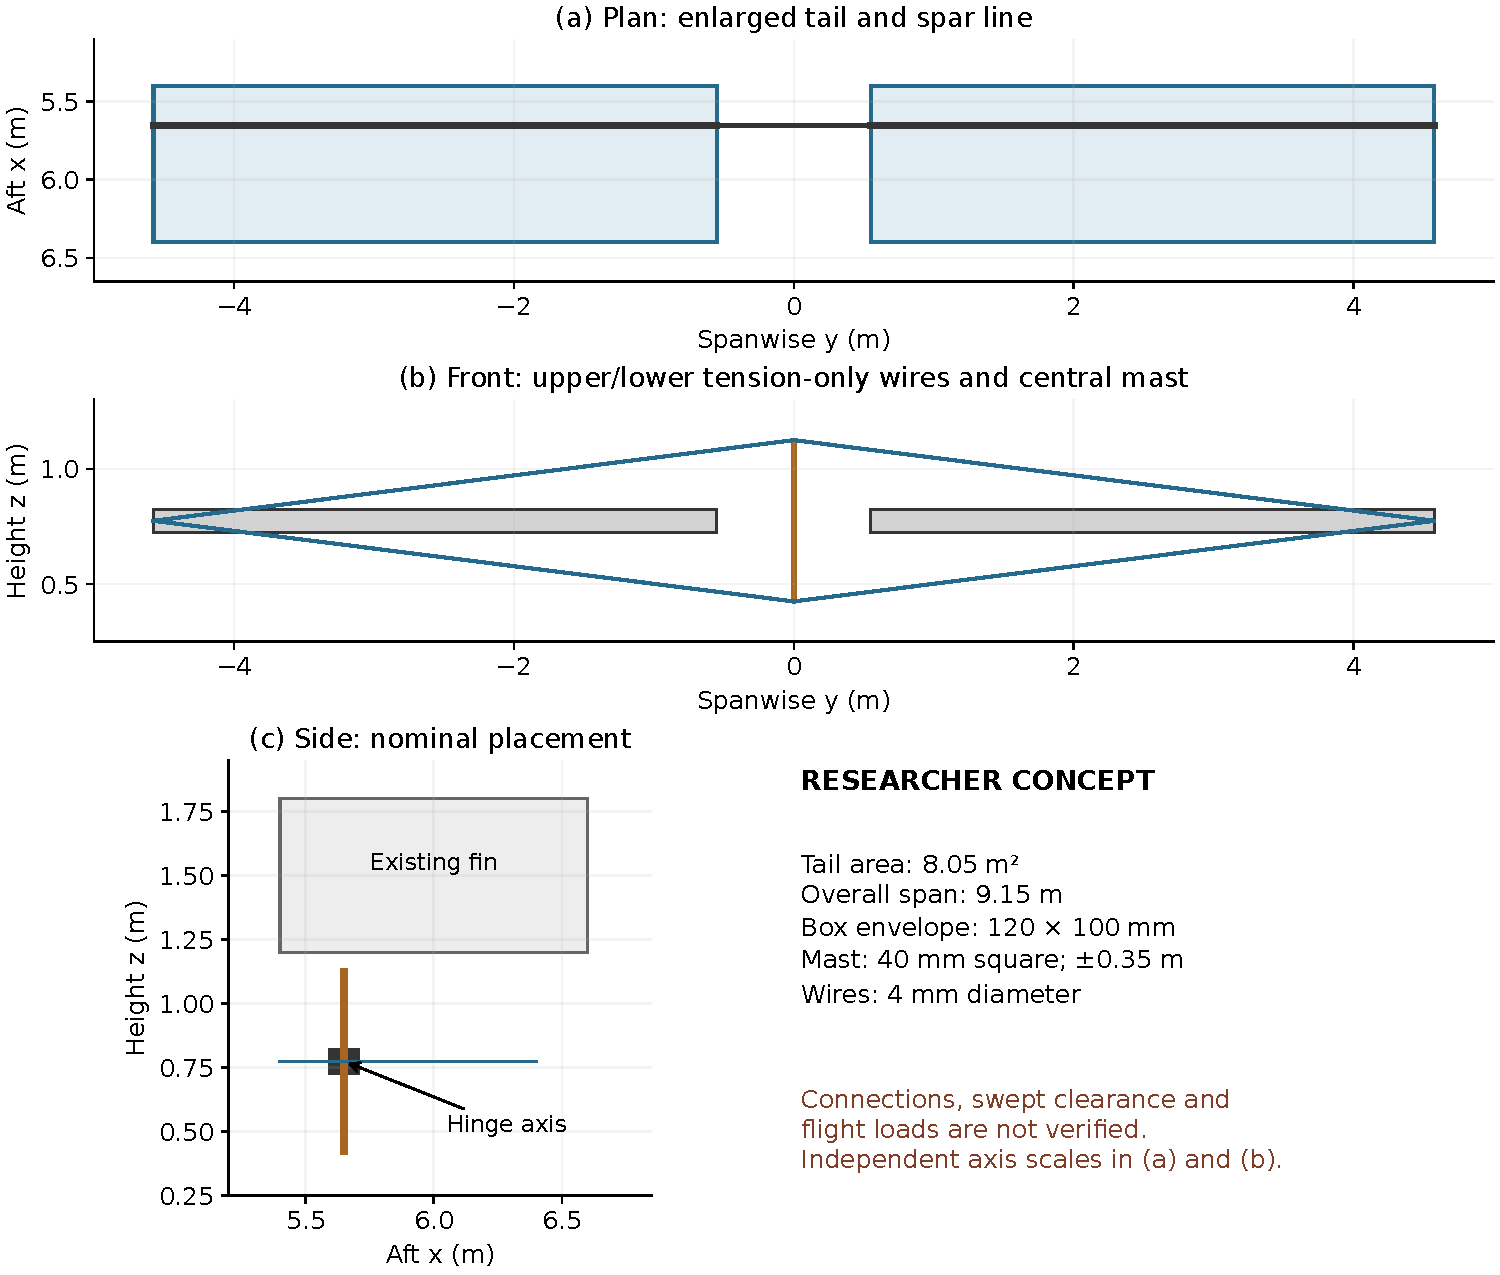
\includegraphics[width=\linewidth]{figures/braced_tail_concept.pdf}
\caption{Researcher braced-tail concept; connections remain unresolved.}
\label{fig:braced-tail-concept}
\end{figure}

The calculation couples a first-order bending beam to geometrically changing,
tension-only wires with zero initial prestress. Wire modulus 200 GPa and
density 7850 kg/m$^3$ are explicit evaluator assumptions, not identified or
certified wire properties. A wire is inactive when its computed extension
would place it in compression. At the evaluated downward load, the upper
wire is active and the lower wire is slack. The displacement compatibility
equation was solved without assigning compressive capacity to the slack wire.
The resulting tip displacement is 11.49 mm, compared with 39.80 mm for the
same box beam without bracing. The corresponding root moment is 139.21 N m
and upper-wire tension is 487.89 N. Multiplying the current strip loads and
weight by three gives 32.43 mm and 1417.29 N; this is only a load-scaling
exercise, not a derived 3-g flight load case. Beam-column effects, local
buckling, joint slip, load reversal, torsion and flutter remain outside the
model. Ideal Euler comparisons do not close those checks.

The calculated masses of the two boxes, four wires and mast are 6.116,
1.810 and 0.502 kg, respectively. Their sum, 8.429 kg, leaves 5.571 kg within
the earlier 14 kg tail allocation for ribs, covering, fittings, horns,
bearings and fasteners. That remainder is a mass budget, not a completed bill
of materials. The original assumed 14 kg ledger has therefore not been
replaced by a supposedly verified structural mass, and the earlier positive
static-margin prediction cannot be claimed for a fully integrated braced
airplane. This branch supplies explicit dimensions and testable requirements
for the next design iteration while retaining the failed additive-beam branch
as evidence of the coupled mass--stability problem.



\subsection{V16 responses and independent loading-envelope checks}
\label{sec:v16_update}
The following results extend, rather than replace, the preceding version history.
All three V16 model responses were eventually received completely. Astra and Opus
completed their first requests; Fable required separately preserved attempts after
output truncation, a transport timeout and an invalid-request response. Its final
request retained the scientific input but required a compact, complete JSON response.
Consequently, response-format instructions and compute expenditure were not identical
across the models. This is a limitation of comparisons of model efficiency, and not
evidence of an engineering advantage. Transport completion is not design acceptance.

Fable's V16 candidate adopts and modifies the evaluator's enlarged, tension-braced
tail. The model selects a continuous 100 by 80 mm box spar with 3.5 mm walls, two
bracing masts at span stations $y=\pm0.55$ m, and upper and lower tie wires. It moves
the nominal pilot centroid forward to $x=0.10$ m and selects a 21.1 kW engine target.
These are model-authored choices following researcher feedback, not independent
rediscovery of the researcher's concept. Summing the 31 printed mass rows gives
365.106 kg and nominal $x_{\rm CG}=1.590720$ m. The reported centroid differs by
approximately 0.13 mm; this arithmetic discrepancy is small relative to the
unverified component-mass uncertainty. The assumed mass ledger is not a weighed
aircraft or a verified manufacturing bill of materials.

Eight loading conditions were independently re-trimmed at 13 m/s on the corrected
fine-grid surface model, using each case's recomputed mass and centroid and the
8.05 m$^2$ tail. Table~\ref{tab:v16_cases} gives the resulting angle of attack,
absolute tail incidence and local surface-model static margin. Unlike the model's
fixed-neutral-point estimates, these margins use $-C_{m_\alpha}/C_{L_\alpha}$ at
the newly solved equilibrium. The largest discrepancy between printed lift and
weight is 0.020 N, and the printed pitching-moment coefficient rounds to zero.
All eight tail incidences lie inside the declared $-16$ to $+8$ degree interval.
The minimum margin is 3.978\%; the exploratory 3\% screening target is not a safety
standard or a quantified uncertainty allowance.

\begin{table}[htbp]
\centering\small
\caption{V16 Fable surface-model equilibria at 13 m/s.}
\label{tab:v16_cases}
\begin{tabular}{rrrrrrr}
\hline
Pilot (kg)&Seat $x$ (m)&Fuel (kg)&Mass (kg)&$\alpha$ (deg)&Tail (deg)&SM (\%)\\
\hline
75 & 0.10 & 8 & 365.106 & 6.026 & -0.661 & 7.006 \\
75 & 0.15 & 8 & 365.106 & 5.986 & -0.483 & 6.423 \\
75 & 0.05 & 8 & 365.106 & 6.065 & -0.839 & 7.589 \\
75 & 0.10 & 0 & 357.106 & 5.733 & -0.621 & 7.039 \\
65 & 0.15 & 8 & 355.106 & 5.465 & 0.262 & 4.006 \\
65 & 0.15 & 0 & 347.106 & 5.174 & 0.302 & 3.978 \\
85 & 0.05 & 8 & 375.106 & 6.600 & -1.637 & 10.031 \\
85 & 0.05 & 0 & 367.106 & 6.305 & -1.597 & 10.122 \\
\hline
\end{tabular}
\end{table}

These results are restricted to rigid lifting surfaces with the inherited,
unvalidated section representation. The calculation omits installed propulsion,
body, landing-gear, mast, wire and fairing forces. Tail control rotates panel normals,
not the physical vertices about the hinge. Thus simultaneous lift and pitch balance
in this model is not installed six-component trim; neither lateral equilibrium under
power nor accepted dynamic modes follows from the positive longitudinal margins.

Independent geometry checks also prevent premature acceptance. Across the full
tail travel, the zero-thickness chord-line envelope includes $x=5.400$ to 6.400 m,
whereas the response reported 5.410 to 6.371 m, excluding the zero-angle position.
Using the rotation sign consistent with the reported vertical envelope, the mast-top
centre spans $x=5.553527$ to 5.698711 m and its bottom spans 5.601289 to 5.746473 m.
The response assigned the same range to both. Correcting these centreline envelopes
does not establish solid clearance: thickness, fittings, body geometry and deflection
must still be included. No collision is claimed from the envelope discrepancy alone.

The other responses likewise require independent qualification. Astra's one-cell
propeller calculation was reproduced and refined to 128 radial cells while retaining
its assumed polar and uniform induction. At 15 m/s, predicted shaft demand increases
from 16.618 to 18.040 kW, leaving only 0.960 kW below its assumed 19 kW ceiling.
This numerical-resolution effect is not a measured propeller correction. In Opus,
a 192-cell calculation at 13 m/s and 500 rpm gives 18.953 kW, above the selected
17.46 kW shaft target. An assumed constant crank torque of 107.43 N m gives a
conditional equilibrium at 483.886 propeller rpm, 16.897 kW and 896.997 N thrust;
an alternative constant-shaft-power assumption gives 488.406 rpm and 921.669 N.
Neither assumed engine characteristic is an available engine map. Same-speed drag
for the revised aircraft, installation effects, tip losses and measured section data
remain missing, so these equilibria do not establish level-flight capability.

The V16 raw responses, evaluator scripts, individual solver outputs and checksum
records accompany this local draft. They have not yet been incorporated into the
immutable public release cited elsewhere. The earlier unresolved structural,
propulsive and dynamic-mode requirements remain open.


\subsection{V16 speed and power sensitivity after surface re-trim}
\label{sec:v16_power_speed}
The apparent power closure in the Fable response is sensitive to the induced-drag
representation. An evaluator-only sensitivity calculation replaces the response's
printed induced-drag coefficient with the fine-grid surface result at the same
speed and mass. It preserves the response's remaining drag assumptions and infers
its propeller efficiency from the printed drag, speed and shaft demand. Consequently,
this calculation does not add two induced-drag estimates, fit an engine map, or
claim a new installed-aircraft equilibrium. With $D_0$ and $P_0$ denoting the printed
total drag and shaft demand for each case, the substitution is
\begin{equation}
\eta_{p,0}=\frac{D_0 V}{P_0},\qquad
D_h=D_0+\tfrac12\rho V^2 S(C_{D_i,s}-C_{D_i,0}),\qquad
P_h=\frac{D_h V}{\eta_{p,0}}
\end{equation}
Here the subscript $s$ identifies the lifting-surface solution and $h$ identifies
the hybrid sensitivity result. Density is 1.225 kg/m$^3$ and reference area is
42 m$^2$. The inferred heavy-case efficiency is approximately 0.45, not a measured
propeller efficiency. The available shaft power remains the response's assumed
$0.95(21.1)=20.045$ kW. Table~\ref{tab:v16_speed_power} compares the three heavy
cases, each at 375.106 kg and the same mass distribution.

\begin{table}[htbp]
\centering\small
\caption{Heavy-case conditional surface and power results; not an accepted operating envelope.}
\label{tab:v16_speed_power}
\begin{tabular}{rrrrrr}
\hline
$V$ (m/s)&$\alpha$ (deg)&$C_{D_i,s}$&$P_h$ (kW)&Reserve (\%)&Headroom (kW)\\
\hline
12 & 9.094 & 0.079577 & 16.362 & 22.51 & 3.683\\
13 & 6.600 & 0.058103 & 18.053 & 11.03 & 1.992\\
16 & 1.902 & 0.026329 & 26.037 & -23.01 & -5.992\\
\hline
\end{tabular}
\end{table}

Reserve is $20.045/P_h-1$; headroom is $20.045-P_h$ in kW. At 13 m/s,
the response's 17.356 kW increases to 18.053 kW. The resulting 0.716 kW shortfall
against $1.15P_h$ must not be confused with an absolute power deficit: the assumed
available power still exceeds demand by 1.992 kW. The 15\% requirement is an
exploratory project screen, not an airworthiness standard. In the nominal
365.106 kg case at the same speed, the analogous substitution gives 13.607 kW.

Two additional fine-grid surface calculations at 12 and 16 m/s converged in lift
and pitch moment with absolute tail incidences of $-2.239$ and $-0.595$ degrees.
Their local surface margins are 10.850 and 8.713\%, respectively. Printed lift
residuals are less than 0.015 N; raw geometry, force and stability hashes were
checked. Speed enters the lift target, without measured Reynolds-dependent
section data. At 12 m/s, $C_L=0.99302$ and $\alpha=9.094$ degrees do not demonstrate
attached flow or adequate stall margin. Lower speed therefore cannot be declared
a solution simply because the assumed shaft-power budget improves. At 16 m/s,
the hybrid demand exceeds the assumed available power by 5.992 kW even though
the restricted lifting-surface equations balance.

These results expose the remaining coupling problem rather than close it.
Propulsion changes force and moment balance, and a larger engine changes mass,
centroid and required lift. The present substitution performs neither feedback
loop. It also leaves the body and bracing drag assumptions, slipstream, thrust-line
moments, section validity and structural deformation unresolved. An accepted
speed envelope requires these effects and stall/control limits to be reconciled
at common operating points. No dynamic-mode or flight acceptance is inferred.

\section{Discussion: What the Wright Comparison Actually Shows}
\subsection{Canard, posture and propulsion are coupled decisions}
Wilbur's 1901 account explicitly links the prone pilot to reducing resistance and describes the forward surface in relation to the movement of pressure on the main supporting surface \cite{ref2}. The same account describes discovering errors in earlier aerodynamic expectations and revising the apparatus. This is evidence of an experimental reasoning process, not proof that a forward elevator is inherently stable. The control patent documents a later specified mechanism, with filing and publication dates after the present input cutoff \cite{ref3}; it is not evidence that the models received that mechanism.

The twin counter-rotating pusher arrangement addresses several coupled issues: reaction torque, propeller diameter and clearance, transmission, pilot/engine placement and the flow encountered by the blades. Aft placement is not universally more efficient. Historical explanations and later aerodynamic interpretations must be attributed separately \cite{ref5,ref6,ref11}. Fable shares the twin, opposite-rotation pusher choice; Astra and Opus V1 also use pushers. Astra V2 instead proposes a tractor, an explicit design-cycle change, not a property of the evaluated V1. The primary divergences are therefore the distribution of lifting area, forward versus aft pitch-control surfaces, seated versus prone posture, and the mechanisms used to correct disturbances.



The models' written rationales can be compared with the engineering consequences of their choices, but they do not reveal the causal origin of those choices. Some responses acknowledge recollection of later aircraft knowledge. Without controlled changes to input information and repeated trials, an assertion that a model ``derived'' a conventional arrangement from nineteenth-century evidence would exceed the experiment. An aft tail is not automatically an anachronism either: the relevant question is the dated evidence and particular implementation, not resemblance to a modern category.

\subsection{Why a good static margin is not the Wright achievement}
Lawrence and Padfield's comparison of the 1903 and 1905 Flyers provides a particularly useful warning \cite{ref10}. Their representation of the later aircraft has a more unfavorable static measure but a slower unstable pitch response and improved control characteristics. Their reported pitch-mode doubling times are approximately 0.41 s for the 1903 representation and 2.192 s for 1905. These are properties of their models and conditions, not measured time constants of the present reconstructions. Their sign convention for the reported static measure must not be copied as the conventional positive-stable margin.

Consequently, ``at least as stable as Wright'' is ambiguous. One endpoint is passive restoring tendency over a specified CG and operating envelope. Another is the ability of a specified pilot/controller to keep a dynamically unstable vehicle within acceptable limits using available controls. The latter also depends on damping, control effectiveness, time delay, actuator limits and workload. Neither endpoint follows from a drawing or a single $C_m=0$ point. The present evidence supports only conditional local pitch diagnostics and identifies the missing inputs for a stronger comparison.

\subsection{What feedback has accomplished, and what it has not}
The Wrights accumulated measurements and piloting experience; this project has so far accumulated descriptions, clarification responses and evaluator calculations. Those are not equivalent experimental resources. The appropriate analogy is the sequence of a falsifiable proposal, test, discrepancy and recorded change. It is not the claim that requesting a revised paragraph recreates the Wrights' learning process.

Self-Refine formalizes iterative textual feedback \cite{ref30}, and Reflexion describes retaining feedback in agent memory \cite{ref32}. Neither constitutes evidence of aerodynamic correctness. Findings on limitations of intrinsic self-correction further motivate feedback grounded in independent calculations rather than assurances of improvement \cite{ref31}. A continuation of the present study must keep those distinctions visible.

Three V2 requests formed a separate researcher-assisted treatment. They retained the original packet and each model's own V1 response, added labelled \emph{modern} conditional numerical evidence, and required changed geometry, mass ledger, controls, propulsion and structural definition. Astra received its destabilizing slope and mechanism gaps; Fable its interference and missing power evidence; Opus its tail load, thrust-line moment and conditional power deficit. No architecture was dictated. Astra replaced its tandem pusher architecture with a fixed wing, aft tail and tractor, so a change in its calculated pitch slope could not be attributed to one isolated design variable. Fable split its tail and moved the fin, directly targeting the identified geometric collision, but its installed drive remains unknown. Opus lengthened its skids, shifted its booms and rudder, and proposed a lower-speed state to address clearance and power concerns. These are documented design responses, not verified performance improvements. Astra and Opus V2 received independent conditional longitudinal retrims, but not complete six-component whole-aircraft trim or validation; Fable's geometry reconciliation remains a prerequisite. The three V2 aircraft are therefore not counted as demonstrated flight-capable revisions.

\subsection{Where this study sits in an iterative aircraft-design cycle}
An aircraft is not designed by drawing its outline once and then checking the wing alone. A mission requirement suggests a configuration and an initial mass; that mass sets a lift requirement; meeting it changes wing area, drag and structural weight; the revised loads and component positions move the CG; and that movement changes the tail force, control travel and thrust-line moment needed for trim. Propulsion sizing, structure, launch and landing must be reconsidered after each significant change. Roskam's modern airplane-design volumes organize these linked tasks as preliminary sizing, configuration and propulsion integration, component-weight estimation, and aerodynamic/thrust/power estimation \cite{ref36,ref37,ref38,ref39}. We use that framework as a present-day audit checklist. It was not part of the pre-1899 packet supplied to the models, and we have not completed every stage of a Roskam design.

In this study, the common historical task produced three V0 arrangements. The V1 clarification provided component coordinates and mass ledgers; we checked the arithmetic of the declared masses and CGs, represented interacting lifting surfaces, solved selected longitudinal balances, tested a control interference and audited whether enough structural detail existed to calculate strength. These are not independent mass estimates, a measured drag build-up, a propeller map, a load-tested structure or a takeoff calculation. Each failed or uncertain check generated a specific V2 feedback request. The new V2 aircraft have \emph{not} been passed back through the same independent whole-aircraft gate. A further V3 request asked for integrated mass, controls, propulsion and flight-dynamics research schedules. The three completed returns passed a provenance and mass-ledger arithmetic audit (Table~\ref{tab:v3returns}), but the two initially token-truncated Claude outputs required separately recorded high-token retries. Fable's stated nominal vertical-force and pitching-moment sums close algebraically; its forces, static margin and derivatives are not independently established. Astra and Opus did not provide complete numerical trim solutions. No V3 return supplies a verified installed derivative set or longitudinal and lateral modal roots. A complete next loop must first reconcile and render each revised geometry, then estimate total drag with uncertainty, solve powered and power-off trim over an admissible angle/control range, compare required power with an installed engine--propeller map, quantify roll/yaw control and structural loads, and repeat after any material change. The present study reports the completed steps and stopping point; it does not fill the remaining steps by assuming that revised model prose is true.

\paragraph{Post-analysis integrated V3 returns.}
The case-specific V3 prompts requested a new complete-aircraft proposal and a
flight-dynamics evidence plan, not an assurance of flight. Astra completed on
the first bounded call. Fable and Opus were cut off at the caller's 20,000-token
output limit; the incomplete responses were retained, and independent
full-prompt retries at a 48,000-token limit returned complete texts. The
structured mass ledgers below were re-summed from their individual entries
with $M=\sum_i m_i$ and $\mathbf{x}_{CG}=\sum_i m_i\mathbf{x}_i/M$.
The native longitudinal axes differ, so $x_{CG}$ values must not be compared
without frame transformation. The returned masses and coordinates are
model assumptions, not measurements. All request and response hashes and the
arithmetic auditor are in the public archive. No V3 numerical result below
replaces the independently computed V1/V2 results in the main analysis.

\begin{table}[H]\centering\footnotesize
\caption{Completed V3 model returns and limited independent arithmetic gate. CG coordinates are in each model's native frame, in metres. ``Force/moment closure'' means arithmetic consistency of the model's stated loads only; it is not an independently predicted aerodynamic trim. No candidate has an independently established installed derivative set, complete longitudinal/lateral roots, or flight acceptance.}\label{tab:v3returns}
\begin{tabularx}{\linewidth}{lXXX}\toprule
Return & Recomputed mass and CG & Nominal force/moment evidence & Full dynamic verdict\\\midrule
Astra V3-I & 333.0 kg; $(-0.150889,0,0.218445)$ & Actual powered/glide trim unknown & Roots unknown; not assessed\\
Fable V3 & 309.5 kg; $(1.556656,0,0.765670)$ & $3245-209-3036=0$ N; $-1329+436-14+907=0$ N m, using assumed loads & Reduced estimates only; not assessed\\
Opus V3 & 361.3 kg; $(0.622676,0,0.460036)$ & Trim left to evaluator by model & Lateral roots unknown; not assessed\\\bottomrule
\end{tabularx}
\end{table}

\subsection{Source-restored feedback and the present stopping point}
The V3 responses were subsequently challenged on component geometry, ground contact and shaft-power arithmetic. V10 corrected several calculations but did not provide a new installed-aircraft geometry. In a first V11 request, we supplied each model only the hash of its archived response and a brief defect summary. All three returned HOLD because a hash cannot reconstruct a component ledger. We retained this unsuccessful request as a protocol error rather than counting it as a model design failure. A second request (V11b) supplied the full V3 and V10 texts, froze their hashes and permitted either an explicit candidate patch or HOLD. All six responses, including the initial unsuccessful round, are retained in the archive.

\begin{table}[H]\centering\small
\caption{Disposition of the source-restored V11b feedback. ``Candidate'' means a model-proposed change whose stated arithmetic was checked; it does not mean flight acceptance. No V11b result is substituted into the V1/V2 trim figures.}\label{tab:v11b}
\begin{tabularx}{\linewidth}{@{}p{16mm}p{31mm}X@{}}\toprule
Model & Response & Independent gate finding\\\midrule
Astra & HOLD; no component change & The parent mass ledger is available, but the truss, bracing, controls and gear are not occupied-solid definitions. Coupling, hinge and ground-sweep compatibility cannot yet be closed.\\
Fable & Seat/gear candidate & A 0.3 kg rail stop restricts seat datum to $x=0.20$--$0.30$ m; new assumed wheel radius and axle coordinates interpret the existing ground contacts. Eight revised mass/CG cases close arithmetically. Loaded gaps, neutral point and available shaft power remain unknown.\\
Opus & HOLD; no component change & Engine-bay physical occupancy and skid contact remain unresolved. The assumed 13.7 kW high-case shaft demand exceeds its unverified 13 kW target; a 15\% reserve would need 15.755 kW measured at the relevant operating point.\\\bottomrule
\end{tabularx}
\end{table}

For Fable, the new nominal ledger gives 309.8 kg and $x_{CG}=1.5312$ m; the light/aft/empty and heavy/forward/empty cases give 283.8 kg at $x_{CG}=1.5854$ m and 303.8 kg at $x_{CG}=1.4728$ m, respectively. Those eight loading cases and the 12 kg gear subdivision reproduce the model's rounded first moments. They are not measured masses or an installed neutral point. In particular, subtracting the aft CG fraction from the model's unvalidated neutral-point estimate to obtain approximately 5.3\% chord does not establish a physical static margin. The assumed nominal 426 N drag at 13 m/s and 0.50 propulsive efficiency requires 11.076 kW at the shaft; 15\% reserve raises the requirement to 12.737 kW. Fable raised its \emph{target} to 12.8 kW but supplied no available-power curve. Its own 14.820 kW sensitivity would require 17.043 kW with the same reserve and therefore fails that target. This difference between a paper power allowance and a measured continuous engine--propeller operating point is decisive.

Opus's new HOLD is also not accepted without scrutiny. Its $0.55$ m-long E1 ledger box centred at $x=0.25$ m spans $x=-0.025$ to $0.525$ m, not $0$ to $0.5$ m as written. The corresponding E1--E3a box intersection is $0.000375$ rather than $0.0003$ m$^3$. More importantly, these ledger boxes may be inertia approximations rather than occupied solids; overlapping approximations alone do not prove that physical engine and tank hardware collide. Thus the valid conclusion is that the engine-bay installation remains undefined, not that collision has been demonstrated. Astra likewise cannot turn an equivalent-mass truss box into member-level clearance evidence. These distinctions preserve the useful feedback while preventing an arithmetic error or pictorial proxy from becoming a flightworthiness claim.

The next feedback made non-minimal physical changes permissible and supplied all earlier model texts. Astra again returned HOLD without a member-resolved installation. Fable proposed a heavier engine, cooling system, drive, fuel arrangement and revised seat stops, but its 26 component rows totalled 354.3 rather than the claimed 353.8 kg. A targeted V13 answer retained every component row and corrected the SUM and eight pilot/seat/fuel cases; our independent ledger gives $m=354.3$ kg and $\boldsymbol r_{CG}=(1.530739,0,0.792233)$ m in its own aft-positive frame. This is bookkeeping closure, not a measured mass. The same audit exposed a more consequential power-chain distinction. Let $\eta_p$ denote the assumed useful-to-propeller-shaft efficiency and $\eta_g$ the assumed engine-to-propeller drive efficiency. For drag $D$ at speed $V$, the minimum engine-side output for a stated 15\% reserve is
\begin{equation}\label{eq:drivegate}
P_{e,\min}=\frac{1.15DV}{\eta_p\eta_g}.
\end{equation}
Under Fable's own heavy/worst-case assumptions, independent recomputation gives 20.047 kW at the engine without engine-mass growth, whereas its retained target is 19.5 kW. The assumed 0.95 drive delivers 18.525 kW to the propeller shafts, 0.520 kW below the 19.045 kW reserved shaft requirement. Holding the 19.5 kW engine target would instead require a drive efficiency of 0.9767, rather than the assumed 0.95. If the model's unverified incremental specific engine mass of 5.1 kg/kW is coupled back into its own drag equation, the paper target rises to 20.195 kW and adds 3.543 kg to the heavy-case mass. This fixed point is arithmetic, not an available engine: cooling, torque and propeller absorption must be rechecked for any real installation. The retained 20 kg fuel row also gives 198.5 min at the model's assumed 0.31 kg/kWh and 19.5 kW, not its stated 20 min; actual fuel flow and endurance remain unknown.

Opus's first V12 response stopped at the specified output-token limit and is retained as incomplete. A separately logged, source-identical 48,000-token replay \emph{completed} and returned a non-minimal analytical installation candidate. Independent summation of its 30 component rows gives 340.3 kg and $(x_{CG},z_{CG})=(0.703552,0.501227)$ m; four pilot/fuel cases close to reported rounding. Its declared rigid aft-skid pivot produces tail-skid contact at $12.994617^\circ$ nose-up, a $0.221112$ m ventral-corner ground gap and a $0.460962$ m aft propeller-tip gap at that stop. These are rigid coordinate calculations; nose-down contact and all loaded clearances remain untested. The assumed 18 kW engine target and 0.97 drive efficiency would give a paper 17.460 kW propeller-shaft target, 1.705 kW above its assumed high-case requirement including 15\% reserve. That arithmetic does not show that a real engine supplies it or that the unspecified propeller absorbs it and produces sufficient thrust. The new Opus CG also lies about 0.081 m aft of its V3 claim, so earlier local stability estimates cannot be carried forward. The complete source and arithmetic gate is archived separately from the first truncated output.

\subsection{Latest-candidate rigid ground-contact screen}
After Fable's V13 mass correction, the V12 nominal ground-load line based on
353.8 kg is superseded. For its declared front-pair and rear contact stations
$x_f=0.40$ and $x_r=3.20$ m, respectively, static equilibrium gives
\begin{equation}\label{eq:groundreactions}
R_f=mg\frac{x_r-x_{CG}}{x_r-x_f},\qquad R_r=mg-R_f
\end{equation}
where $R_f$ is the total front-wheel reaction and $R_r$ the rear reaction.
Independent recomputation of all eight declared V13 mass/CG states gives
positive reactions. The nominal 354.3 kg state gives 2072.079 N at the front
pair and 1403.604 N at the rear; across the cases these range from 1846.975
to 2188.572 N and from 1301.125 to 1418.494 N, respectively. In a rigid
nose-down rotation about the front contact line, the specified skid point
contacts at $20.556^\circ$; this does not cover tire compression, braking,
or an occupied-solid sweep.

For Opus V12, the specified front upturn of the flat runner contacts the
ground at $41.186^\circ$ nose-down in a rigid rotation about the front end
of the flat segment. A specified lower/front nacelle-box corner would reach
ground later, at $79.216^\circ$ under the same idealization, and all four
reported longitudinal CG projections lie between the flat-runner endpoints.
These selected-point checks do not establish the first contact of the entire
occupied, loaded aircraft or the distribution of load along the runner.
Astra V12 supplies no adopted installed geometry for the corresponding test.
The exact source hashes, inputs and all Fable cases are recorded in the frozen
ground-contact audit; none of these ground results is a flight-stability
derivative.

\subsection{Nominal installation-gap screen}
Fable V13 explicitly retained the V12 occupied geometry. From its declared
coordinate intervals, six one-axis rigid separations were independently
recomputed; the smallest is only 0.010 m between the tank top and upper
longeron. The engine-to-frame side gap is 0.020 m and the nominal inboard
propeller-disc-to-frame gap is 0.050 m. Opus V12 itself reports selected
0.010--0.050 m gaps near the engine/shaft, bearer/wing, gear and control
interfaces, but these have not been independently reconstructed as complete
three-dimensional solids. A positive nominal gap is not a loaded or swept
clearance: thickness, assembly tolerances, propeller motion, structural
deflection and control travel are unbounded. The source-hashed one-axis
calculations and model-reported values are kept separate in the clearance
audit. No aircraft passes the installed-geometry gate on these data.

\subsection{Centroid-only inertia screen}
For the latest complete Fable V13 and Opus V12 mass ledgers, the evaluator
assembled the parallel-axis contribution
\begin{equation}\label{eq:parallelaxis}
\mathbf J_{\mathrm{parallel}}=\sum_i m_i
\left[(\mathbf d_i\cdot\mathbf d_i)\mathbf I-\mathbf d_i\mathbf d_i^T\right],
\qquad \mathbf d_i=\mathbf r_i-\mathbf r_{CG},
\end{equation}
from declared component-centroid locations. The diagonal contributions, in kg m$^2$, are
\begin{align*}
\text{Fable:}\quad (J_{xx},J_{yy},J_{zz})&=(282.406,522.525,668.278),\\
\text{Opus:}\quad (J_{xx},J_{yy},J_{zz})&=(131.713,914.293,782.580).
\end{align*} These are conditional
lower bounds, not measured aircraft inertias. The actual tensor also contains
the unknown intrinsic tensor of every component, including pilot, wings,
engine and propellers. The complete matrices, coordinate convention and
source hashes are in the evaluator's inertia audit. Astra V12 has no adopted
installed ledger. No modal eigenvalues are computed from these incomplete
tensors; aerodynamic rate and unsteady derivatives are also missing.

\subsection{Which generated design is strongest on present evidence?}
The comparison is between \emph{three V1 aircraft proposals under the same evaluator}, not a statistical ranking of the underlying language models. A useful decision rule gives priority to (i) an explicitly reconstructible mass and geometry, (ii) an admissible longitudinal balance, (iii) a restoring local fixed-control pitch response, and (iv) no known geometric contradiction at the balancing control setting. Installed power, full-axis control and strength remain required gates, so passing these four screens cannot establish flight.

On this restricted rule, \emph{Opus V1 is the strongest evaluated initial proposal}. Its direct fine-grid balance has a small evaluated moment residual, its wing decks and aft tail supply a coherent lift/downforce and pitching-moment budget, and its lifting-surface-only $C_{m_\alpha}<0$ corresponds to an effective local margin near 5\% of its declared reference chord. Its known weakness is the sensitive 13.35 kW demand relative to an unverified 13 kW target under $\Delta C_D=0.05$ and $\eta=0.60$; changing either assumption can change that verdict. Moreover, body, propeller wake, pilot and structural effects could alter its apparent static margin. Astra V1 also admits conditional trim, but its positive fixed-control $C_{m_\alpha}$ is destabilizing in the retained representation, and its long-shaft/control load paths are incomplete. Fable V1 shares the Wrights' twin counter-rotating pusher choice and has a light declared mass, but every sampled mathematical trim requires motion of a continuous tail through its fixed fin. That geometric conflict prevents treating those roots as operable states.

For the \emph{latest V2 designs}, Astra has the strongest \emph{conditional longitudinal} screen among the two independently retrimmed aircraft: its calculated margin is 19.47\% versus Opus's 7.76\%, and its estimated engine demand is 8.46 kW versus an 18 kW target, compared with Opus's 11.67 kW versus 13 kW. Both power comparisons rely on unverified targets, different speeds and assumed drag/efficiencies. A large static margin is not automatically better handling, and Astra's wholesale conversion to a tractor, fixed-wing/aft-tail layout reduces causal attribution to feedback and raises new propeller reaction/control questions. Fable V2 is not an independently trimmed comparator. Thus Astra is the most promising \emph{V2 candidate for further testing on these particular screens}, while there is no defensible overall winner for actual flightworthiness. None is shown superior to the historically flown Flyer I in controllability or flight capability; the experimental budgets and evidence classes differ.

\subsection{Detailed integrated design-return records}

\begin{table}[H]\centering\footnotesize
\caption{V1 architectural comparison and remaining evidence.}\label{tab:architecture}
\begin{tabularx}{\linewidth}{l*{4}{>{\raggedright\arraybackslash}X}}\toprule
System & Wright 1903 & Astra & Fable & Opus\\\midrule
Lifting layout & Main biplane, forward elevator & Tandem lifting surfaces & Biplane, aft tail & Biplane, aft tail\\
Pilot/control & Prone; mechanical pitch, warping and yaw controls & Seated; collective/differential forward incidence & Seated; movable tips and rotating tail & Seated; flaps, elevator and rudder\\
Propulsion & Twin counter-rotating pushers; historical operation & Pusher with long shaft; installation unverified & Twin counter-rotating pushers; available power unresolved & Pusher; conditional power margin inadequate at selected efficiency\\
Structure & Historical built artifact; later replicas require separate identity & Truss/wing-root and bearing paths incomplete & Lattice/member and joint definition incomplete & Spar/strut/wire definition incomplete\\
Evidence & Documented flights, later tests and reconstructions & Numerical conditions only & Mechanical conflict in sampled trims & Numerical conditions only\\\bottomrule
\end{tabularx}
\end{table}


\subsection{Retained earlier configuration comparison}
This earlier V1 comparison plate is retained alongside the updated presentation to preserve the complete drawing record. It does not describe the latest V15 installation.
\begin{landscape}\begin{figure}[H]\centering
\includegraphics[width=.96\linewidth,height=.76\textheight,keepaspectratio]{\figdir/configuration_comparison_v2.png}
\caption{Earlier V1 configuration-comparison plate retained from the complete September 27 manuscript.}\label{fig:earliercomparison}
\end{figure}\end{landscape}

\section{Limitations and Reproducibility}
The principal limitations are physical, not typographic: total drag and installed propulsion are unvalidated; the lifting model excludes separated flow and flexibility; complete structural and inertia definitions are absent; lateral/directional response has not been established; and the Wright reference is not fully matched to a sourced CG and as-tested configuration. A positive result from the current evaluator would remain a conditional screening result.

The design experiment itself is small and exploratory. Unequal budgets, model-specific clarification and incomplete historical request recovery prevent population-level conclusions about models. Supplied-source restriction is not a pretraining cutoff. The literature review is targeted rather than systematic; access levels and claim-to-source notes are retained in an annotated bibliography. References inspected only at abstract or metadata level are not used for uninspected quantitative details.

The tagged public research snapshot contains the locally recovered original prompts, packet text, model responses and failures (including both V3 token-truncated attempts and the completed retries), diagrams, versioned geometry, analysis code, selected inputs/outputs, and a file-level checksum manifest. The archive also identifies what cannot be reconstructed from retained service history. Third-party papers, supplied lecture scans, credentials and unreviewed software binaries are excluded. FAIR principles motivate identifiers, metadata and reuse conditions \cite{ref33}; reproducibility guidance motivates explicit experimental settings and code/data reporting \cite{ref34}. A repository alone, however, is neither physical validation nor a substitute for independent checking.

AI systems generated the evaluated concepts and assisted in analysis and manuscript preparation. They are not authors. The human author retains responsibility for source interpretation, calculations and any submitted version. These computational results do not authorize physical construction or occupied flight; journal claims must retain the stated evidence limits.

\section{Conclusions}
Historically constrained prompting produced three specified aircraft concepts, not three demonstrated flying aircraft. Clarification made their mass, geometry and interfaces more auditable, but it did not establish successful design optimization. Independent calculations now show the individual lifting-surface loads, opposing aerodynamic and thrust moments, and differences between interpolated balances and direct fine-grid results.

Astra V1's local fixed-control pitch tendency is destabilizing in the retained model. Opus V1's lifting-surface-only tendency is restoring, but its representative power demand slightly exceeds an unverified target under researcher-chosen drag and assumed efficiency. Fable V1's sampled trim candidates require mechanically conflicting tail motion. Thus Opus is the most promising \emph{initial V1 proposal} under the stated screens. After feedback, Astra V2 has the largest conditional longitudinal restoring and assumed-power margins of the two retrimmed revisions; Fable V2 remains blocked by definition gaps. Neither phase supports a general ranking of model intelligence or a claim that any design is flightworthy. None of these findings alone proves design-wide impossibility; together they rule out presenting the current set as three validated, stable aircraft.

Later feedback produced a corrected Fable loading ledger, while Astra and Opus retained installation or propulsion holds. The Fable V13 power chain failed its assumed 15\% reserve; the revised V15 paper target passes that particular H13W arithmetic screen, yet fails the H16W case by 4.164 kW and has no measured engine--propeller map. Direct V15 evaluation balances only the modelled wing--tail lift and pitch moment, not the six installed-aircraft components. The original split-tip lift shift was traced to an evaluator component-grouping error. Correcting this setting, the tail command representation and fin/rudder panel alignment permits a new conditional trim and static/control/rate screen; these predictions still do not establish aircraft modes. No design has a verified neutral point, powered/glide six-component trim, complete dynamic derivative set, accepted modes or structural adequacy. These outcomes do not overturn the restricted V1/V2 rankings or identify a flightworthy winner. The Wright comparison strengthens rather than relaxes the evidence standard: historical controlled flight, static restoring tendency and dynamic controllability are different outcomes. Further model prose cannot replace installed propulsion, loaded-clearance and whole-aircraft balance data.

The loading-envelope check further narrows the nominal V15 result: the two light-pilot aft-CG states have negative surface-model margins despite equilibrium. A researcher-generated enlarged tail gives positive margins across eight coarse-grid loading states and two fine-grid critical states, but its structural and control redesign remain unresolved. The explicit added-mass sensitivity shows why aerodynamic restoration cannot be separated from mass and structural closure. This evaluator intervention is not an additional success attributed to Fable, and it does not establish a dynamically acceptable airplane.


The latest V16 result changes the conditional Fable assessment, not the historical
record above. All three responses are now complete, but response completion is not
an engineering gate. The revised Fable mass distribution and enlarged braced tail
give positive surface-model margins across eight loading states at 13 m/s. Its
claimed heavy-case power closure is not robust to replacing the induced-drag
estimate with the corresponding fine-grid result: the reserve falls to 11.0\%.
The 12 m/s power screen is more favorable but has unverified stall margin, while
the 16 m/s case retains a substantial assumed-power deficit. Thus Fable is a
candidate for further coupled analysis, not a flightworthy winner. The decisive
remaining inputs are installed propulsion and drag, loaded geometry and structural
properties, physical inertia, and justified unsteady derivatives. Until those
inputs support common powered and glide equilibria, numerical eigenvalues would
not constitute validated aircraft modes.

\section*{Data availability}
The locally recovered prompts, historical input packet, model responses (including failed, truncated and separately logged retries), versioned geometry, figure source data, and analysis inputs and outputs through V13 are available in the tagged draft research repository \url{https://github.com/Ehsan-Roohi/historical-aircraft-llm/tree/aircraft-joa-2026-09-29-g8-draft}. The original consolidated \texttt{research\_evidence.zip} and \texttt{MANIFEST.json} remain the earlier R5 snapshot; later V9--V13 records and checksums are individually versioned. At this G8 tag, three V14 prompts were frozen as \texttt{FROZEN\_UNSENT}; that status describes only the dated public snapshot. The later V14 and V15 replies, checksums, and independent local screens discussed in this working revision have not yet been incorporated into a new immutable public release. The local review ZIP accompanying this draft contains the V15 lateral-screen, loading-envelope, researcher tail-trade and added-mass sensitivity scripts, inputs, outputs and checksum manifest, but is not a substitute for a fixed public research release containing the complete model conversations. This draft is not submission-ready until those post-G8 records are released and the manuscript is reconciled against them. Unrecorded service-side details are not reconstructed. Third-party books, articles and privately supplied lecture scans are cited but not redistributed. No physical flight, wind-tunnel or measured engine--propeller dataset was generated for the proposed aircraft.


\paragraph{Records added through V16.}
The complete local package for this revision additionally includes the three
complete V16 responses and the independent mass, geometric-envelope, loading,
surface-trim, propeller and speed--power audits under \texttt{audit\_data/v16}.
The speed--power additions are in \texttt{audit\_data/v16/power\_speed} and include
the two raw speed runs, audit scripts and source hashes. The earlier G8 tag remains
unchanged; these local additions must not be represented as publicly released at
that tag. The package preserves earlier manuscript versions by reference to the
unchanged local draft24 and records the replaced abstract in its revision audit.
Bundled calculation scripts retain provenance paths and may require path adaptation
and the separately obtained solver; this is an audit archive, not a claim of a
fully self-contained executable environment. Before submission, the author must
approve a fixed public data/code release and reconcile its identifier with this
statement. Third-party redistribution restrictions remain in force.

\section*{Code availability}
Custom analysis and figure-generation code, with frozen text inputs and outputs, is available at the same fixed tag and is described in Methods. The external AVL executable and copyrighted reference material are not redistributed. The shared code does not remove the unresolved geometry, power, inertia and unsteady-aerodynamic inputs needed for physical validation.

\section*{Acknowledgments and use of artificial intelligence}
The three named language models were the experimental design generators. Their
archived outputs were treated as proposals, not as independent technical
evidence. An OpenAI coding assistant assisted with research organization,
drafting and editing, analysis-code development, and figure production.
Model-assisted prose, calculations, citations, and graphics require author
review; no language model is an author. The human author is responsible for
the submitted scientific claims, source attribution, and figure accuracy.
The same research, writing, and figure uses must also be disclosed in the
ScholarOne submission fields. Funding and conflict-of-interest information
must be confirmed by the author before submission.

\begingroup\raggedright
% Ordered by first citation for AIAA journal style.
\begin{thebibliography}{99}
\bibitem{ref1} Chanute, O., \emph{Progress in Flying Machines}, American Engineer and Railroad Journal, New York, 1894. Digitized book, Library of Congress, LCCN 31015366, \url{https://www.loc.gov/item/31015366/}.

\bibitem{ref2} Wright, W., ``Some Aeronautical Experiments,'' address to the Western Society of Engineers, 18 September 1901; author-revised reprint from the \emph{Journal of the Western Society of Engineers}, December 1901. Wilbur and Orville Wright Papers, Library of Congress, \url{https://tile.loc.gov/storage-services/service/mss/mss46706/mss46706-05001168/mss46706-05001168.pdf}.

\bibitem{ref4} Daniels, J. T., ``First Flight, 120 Feet in 12 Seconds, 10:35 a.m.; Kitty Hawk, North Carolina,'' photograph, 17 December 1903, Library of Congress, item 00652085, \url{https://www.loc.gov/item/00652085/}.

\bibitem{ref5} Culick, F. E. C., ``The Wright Brothers: First Aeronautical Engineers and Test Pilots,'' \emph{AIAA Journal}, Vol. 41, No. 6, 2003, pp. 985--1006. \url{https://doi.org/10.2514/2.2046}. Author repository: \url{https://authors.library.caltech.edu/records/mjnjq-4a740}.

\bibitem{ref35} National Air and Space Museum, ``1903 Wright Flyer,'' Smithsonian Institution collection record, accessed 27 September 2026. \url{https://airandspace.si.edu/collection-objects/1903-wright-flyer/nasm_A19610048000}.

\bibitem{ref8} Kochersberger, K., Ash, R., Britcher, C., Landman, D., Sandusky, R., and Hyde, K., ``An Evaluation of the Wright 1901 Glider Using Full Scale Wind Tunnel Data,'' AIAA Paper 2002-1134, 2002. \url{https://centennialofflight.net/wbh/wr_experience/1901/pdfs/1901.pdf}.

\bibitem{ref7} Padfield, G. D., and Lawrence, B., ``The Birth of Flight Control: An Engineering Analysis of the Wright Brothers' 1902 Glider,'' \emph{The Aeronautical Journal}, Vol. 107, No. 1078, 2003, pp. 697--718. \url{https://doi.org/10.1017/S0001924000013464}.

\bibitem{ref9} Lawrence, B., and Padfield, G. D., ``Handling-Qualities Analysis of the Wright Brothers' 1902 Glider,'' \emph{Journal of Aircraft}, Vol. 42, No. 1, 2005, pp. 224--236. \url{https://doi.org/10.2514/1.6091}.

\bibitem{ref11} Deters, R. W., Broughton, B. A., and Selig, M. S., ``A Retrospective: Development of Simulation Models for the 1903 and 1905 Wright Flyers,'' AIAA Paper 2004-0211, 2004. \url{https://m-selig.web.engr.illinois.edu/pubs/DetersBroughtonSelig-2004-AIAA-2004-0211-WrightFlyers.pdf}.

\bibitem{ref12} Cherne, J., Culick, F. E. C., and Zell, P., ``The AIAA 1903 Wright `Flyer' Project Prior to Full-Scale Tests at NASA Ames Research Center,'' AIAA Paper 2000-0511, 2000. \url{https://www.wrightflyerproject.com/wp-content/uploads/2012/10/The-AIAA-1903-Wright-Flyer-Project-Prior-to-Full-Scale-Tests.pdf}.

\bibitem{ref13} Jex, H. R., Grimm, R., Latz, J., and Hange, C., ``Full-Scale 1903 Wright Flyer Wind Tunnel Test Results From the NASA Ames Research Center,'' slide presentation associated with AIAA Paper 2000-0512, 2000. Wright Flyer Project publication index and download: \url{https://www.wrightflyerproject.com/technical-papers-and-publications/index.html}.

\bibitem{ref16} Raffel, M., Wienke, F., and Dillmann, A., ``Flight-Testing Stability and Controllability of Otto Lilienthal's Monoplane Design from 1893,'' \emph{Journal of Aircraft}, Vol. 56, No. 4, 2019, pp. 1735--1742. \url{https://doi.org/10.2514/1.C035399}.

\bibitem{ref17} Raffel, M., Wienke, F., and Dillmann, A., ``Flying Qualities of Otto Lilienthal's Large Biplane,'' \emph{Journal of Aircraft}, Vol. 58, No. 2, 2021, pp. 413--419. \url{https://doi.org/10.2514/1.C036022}.

\bibitem{ref18} Raffel, M., Wienke, F., Schwarz, C., and Dillmann, A., ``Flight Controls of Otto Lilienthal's Experimental Monoplane from 1895,'' \emph{Journal of Aircraft}, Vol. 59, No. 6, 2022, pp. 1616--1625. \url{https://doi.org/10.2514/1.C037047}.

\bibitem{ref19} Wienke, F., Raffel, M., and Dillmann, A., ``Wind-Tunnel Testing of Otto Lilienthal's Production Aircraft from 1893,'' \emph{AIAA Journal}, Vol. 59, No. 4, 2021, pp. 1342--1351. \url{https://doi.org/10.2514/1.J059831}.

\bibitem{ref25} Tong, Y., Luo, M., Ren, S., Zhang, Z., Xing, C., and Du, Z., ``A Rapidly Structured Aircraft Concept Design Method Based on Generative Artificial Intelligence,'' \emph{Chinese Journal of Aeronautics}, Vol. 38, No. 10, 2025, Article 103629. \url{https://doi.org/10.1016/j.cja.2025.103629}.

\bibitem{ref26} Krus, P., ``Large Language Model in Aircraft System Design,'' \emph{ICAS 2024 Proceedings}, Paper 0514, 2024. \url{https://www.icas.org/icas_archive/icas2024/data/papers/icas2024_0514_paper.pdf}.

\bibitem{ref27} Liu, S., Shen, Y., Zhang, Y., Hou, Z., Wang, X., Luo, J., and Zhang, Z., ``iDesignGPT Enhances Conceptual Design via Large Language Model Agentic Workflows,'' \emph{Nature Communications}, Vol. 17, 2026, Article 1997. \url{https://doi.org/10.1038/s41467-026-68672-1}.

\bibitem{ref28} Samplawski, C., Cobb, A. D., and Jha, S., ``AGENT: An Aerial Vehicle Generation and Design Tool Using Large Language Models,'' arXiv preprint arXiv:2504.08981, 2025. \url{https://arxiv.org/abs/2504.08981}.

\bibitem{ref29} Cobb, A. D., Roy, A., Elenius, D., Heim, F. M., Swenson, B., Whittington, S., Walker, J. D., Bapty, T., Hite, J., Ramani, K., McComb, C., and Jha, S., ``AircraftVerse: A Large-Scale Multimodal Dataset of Aerial Vehicle Designs,'' \emph{Advances in Neural Information Processing Systems}, Vol. 36, Datasets and Benchmarks Track, 2023. \url{https://proceedings.neurips.cc/paper_files/paper/2023/file/8b94879b177d9780c17f5a78f62a6a8a-Paper-Datasets_and_Benchmarks.pdf}.

\bibitem{ref6} Culick, F. E. C., and Jex, H. R., ``Aerodynamics, Stability and Control of the 1903 Wright Flyer,'' accepted report version, AIAA Wright Flyer Project Report WF 84/09-1, Systems Technology, Inc., Paper 359, CaltechAUTHORS record dated 1985. \url{https://authors.library.caltech.edu/records/vea6k-35x13}.

\bibitem{ref43} Ash, R. L., Miley, S. J., Landman, D., and Hyde, K. W., ``Evolution of Wright Flyer Propellers between 1903 and 1912,'' AIAA Paper 2001-0309, 2001. \url{https://www.wrightexperience.com/wp-content/uploads/sites/161/2015/07/Propeller-Evolution.pdf}.

\bibitem{ref41} Papachristodoulou, A. N., and Culick, F. E. C., ``Flight Mechanics of the Wright Aircraft 1903--1912,'' AIAA Paper 2003-0097, 2003. \url{https://authors.library.caltech.edu/records/0vz83-2z634}.

\bibitem{ref42} Padfield, G. D., and Lawrence, B., ``The Birth of the Practical Aeroplane: An Appraisal of the Wright Brothers' Achievements in 1905,'' \emph{The Aeronautical Journal}, Vol. 109, 2005, pp. 421--437. \url{https://pcwww.liv.ac.uk/eweb/fst/publications/2994COL_final_final.pdf}.

\bibitem{ref10} Lawrence, B., and Padfield, G. D., ``Flight Handling Qualities of the Wright Brothers' 1905 Flyer 3,'' \emph{Journal of Aircraft}, Vol. 43, No. 5, 2006, pp. 1307--1316. \url{https://doi.org/10.2514/1.19607}.

\bibitem{ref44} Strauss, M., ``Wilbur and Orville Wright's 1909 Triumph for the U.S. Army,'' \emph{Air \& Space Quarterly}, National Air and Space Museum, Winter 2025. \url{https://airandspace.si.edu/air-and-space-quarterly/issue-13/wright-military-flyer}.

\bibitem{ref20} Drela, M., and Youngren, H., \emph{AVL 3.40 User Primer}, 22 February 2022, retained manual; executed solver version 3.52. Author software and documentation site: \url{https://web.mit.edu/drela/Public/web/avl/}.

\bibitem{ref21} Drela, M., \emph{Flight Vehicle Aerodynamics}, MIT Press, Cambridge, MA, 2014, ISBN 9780262526449. \url{https://mitpress.mit.edu/9780262526449/flight-vehicle-aerodynamics/}.

\bibitem{ref22} Katz, J., and Plotkin, A., \emph{Low-Speed Aerodynamics}, 2nd ed., Cambridge University Press, 2001. \url{https://doi.org/10.1017/CBO9780511810329}.

\bibitem{ref24} Oberkampf, W. L., and Trucano, T. G., ``Verification and Validation in Computational Fluid Dynamics,'' \emph{Progress in Aerospace Sciences}, Vol. 38, No. 3, 2002, pp. 209--272; associated report SAND2002-0529. Sandia record: \url{https://www.sandia.gov/research/publications/details/verification-and-validation-in-computational-fluid-dynamics-2002-03-01/}.

\bibitem{ref15} Anderson, S. B., \emph{A Look at Handling Qualities of Canard Configurations}, NASA TM-88354, September 1986. \url{https://ntrs.nasa.gov/citations/19870013196}.

\bibitem{ref23} Cooper, G. E., and Harper, R. P., Jr., \emph{The Use of Pilot Rating in the Evaluation of Aircraft Handling Qualities}, NASA TN D-5153, April 1969. \url{https://ntrs.nasa.gov/citations/19690013177}.

\bibitem{ref40} Drela, M. and Youngren, H., \emph{AVL User Primer}, Massachusetts Institute of Technology, version 3.36. \url{https://web.mit.edu/drela/Public/web/avl/AVL_User_Primer.pdf}.

\bibitem{ref46} Senalik, C. A., and Farber, B., ``Mechanical Properties of Wood,'' Chapter 5 in \emph{Wood Handbook: Wood as an Engineering Material}, General Technical Report FPL-GTR-282, U.S. Department of Agriculture, Forest Service, Forest Products Laboratory, Madison, WI, 2021. \url{https://research.fs.usda.gov/download/treesearch/62244.pdf}.

\bibitem{ref3} Wright, O., and Wright, W., ``Flying-Machine,'' U.S. Patent 821,393, filed 23 March 1903, granted 22 May 1906, \url{https://patents.google.com/patent/US821393A/en}.

\bibitem{ref30} Madaan, A., Tandon, N., Gupta, P., Hallinan, S., Gao, L., Wiegreffe, S., Alon, U., Dziri, N., Prabhumoye, S., Yang, Y., Gupta, S., Majumder, B. P., Hermann, K., Welleck, S., Yazdanbakhsh, A., and Clark, P., ``Self-Refine: Iterative Refinement with Self-Feedback,'' \emph{Advances in Neural Information Processing Systems}, Vol. 36, 2023. \url{https://doi.org/10.52202/075280-2019}.

\bibitem{ref32} Shinn, N., Cassano, F., Gopinath, A., Narasimhan, K., and Yao, S., ``Reflexion: Language Agents with Verbal Reinforcement Learning,'' \emph{Advances in Neural Information Processing Systems}, Vol. 36, 2023. \url{https://papers.nips.cc/paper_files/paper/2023/hash/1b44b878bb782e6954cd888628510e90-Abstract-Conference.html}.

\bibitem{ref31} Huang, J., Chen, X., Mishra, S., Zheng, H. S., Yu, A., Song, X., and Zhou, D., ``Large Language Models Cannot Self-Correct Reasoning Yet,'' \emph{International Conference on Learning Representations}, 2024. \url{https://proceedings.iclr.cc/paper_files/paper/2024/hash/8b4add8b0aa8749d80a34ca5d941c355-Abstract-Conference.html}.

\bibitem{ref36} Roskam, J., \emph{Airplane Design, Part I: Preliminary Sizing of Airplanes}, DARcorporation, Lawrence, KS, 2018 reprint, ISBN 978-1-884885-42-6. \url{https://shop.darcorp.com/index.php?product_id=51&route=product/product}.

\bibitem{ref37} Roskam, J., \emph{Airplane Design, Part II: Preliminary Configuration Design and Integration of the Propulsion System}, DARcorporation, Lawrence, KS, 2018 reprint, ISBN 978-1-884885-43-3. \url{https://shop.darcorp.com/index.php?product_id=53&route=product/product}.

\bibitem{ref38} Roskam, J., \emph{Airplane Design, Part V: Component Weight Estimation}, DARcorporation, Lawrence, KS, 2018 reprint, ISBN 978-1-884885-50-1. \url{https://shop.darcorp.com/index.php?product_id=55&route=product/product}.

\bibitem{ref39} Roskam, J., \emph{Airplane Design, Part VI: Preliminary Calculation of Aerodynamic, Thrust and Power Characteristics}, DARcorporation, Lawrence, KS, 2008 reprint, ISBN 978-1-884885-52-5. \url{https://shop.darcorp.com/index.php?product_id=56&route=product/product}.

\bibitem{ref33} Wilkinson, M. D., Dumontier, M., Aalbersberg, I. J., Appleton, G., Axton, M., Baak, A., Blomberg, N., Boiten, J.-W., Bonino da Silva Santos, L., Bourne, P. E., Bouwman, J., Brookes, A. J., Clark, T., Crosas, M., Dillo, I., Dumon, O., Edmunds, S., Evelo, C. T., Finkers, R., Gonzalez-Beltran, A., Gray, A. J. G., Groth, P., Goble, C., Grethe, J. S., Heringa, J., 't Hoen, P. A. C., Hooft, R., Kuhn, T., Kok, R., Kok, J., Lusher, S. J., Martone, M. E., Mons, A., Packer, A. L., Persson, B., Rocca-Serra, P., Roos, M., van Schaik, R., Sansone, S.-A., Schultes, E., Sengstag, T., Slater, T., Strawn, G., Swertz, M. A., Thompson, M., van der Lei, J., van Mulligen, E., Velterop, J., Waagmeester, A., Wittenburg, P., Wolstencroft, K., Zhao, J., and Mons, B., ``The FAIR Guiding Principles for Scientific Data Management and Stewardship,'' \emph{Scientific Data}, Vol. 3, 2016, Article 160018. \url{https://doi.org/10.1038/sdata.2016.18}.

\bibitem{ref34} Pineau, J., Vincent-Lamarre, P., Sinha, K., Lariviere, V., Beygelzimer, A., d'Alche-Buc, F., Fox, E., and Larochelle, H., ``Improving Reproducibility in Machine Learning Research (A Report from the NeurIPS 2019 Reproducibility Program),'' \emph{Journal of Machine Learning Research}, Vol. 22, No. 164, 2021, pp. 1--20. \url{https://jmlr.org/papers/v22/20-303.html}.
\end{thebibliography}

\endgroup
\end{document}
